%
% Template Laporan Skripsi/Thesis 
%
% @author  Andreas Febrian, Lia Sadita 
% @version 1.03
%
% Dokumen ini dibuat berdasarkan standar IEEE dalam membuat class untuk 
% LaTeX dan konfigurasi LaTeX yang digunakan Fahrurrozi Rahman ketika 
% membuat laporan skripsi. Konfigurasi yang lama telah disesuaikan dengan 
% aturan penulisan thesis yang dikeluarkan UI pada tahun 2008.
%

%
% Tipe dokumen adalah report dengan satu kolom. 
%
\documentclass[12pt, a4paper, onecolumn, oneside, final]{report}

% Load konfigurasi LaTeX untuk tipe laporan thesis
\usepackage{style/uithesis}
\usepackage{natbib}
\usepackage{import}

% Load konfigurasi khusus untuk laporan yang sedang dibuat
%-----------------------------------------------------------------------------%
% Informasi Mengenai Dokumen
%-----------------------------------------------------------------------------%
% 
% Judul laporan. 
\var{\judul}{Desain dan Analisa Penerapan Pola Model-View-Controller (MVC)
    Untuk Pengembangan Software Product Line (SPL) Berbasis Web dengan
    Menggunakan Bahasa Pemodelan Abstract Behavioural Spesification (ABS)}
% 
% Tulis kembali judul laporan, kali ini akan diubah menjadi huruf kapital
\Var{\Judul}{Desain dan Analisa Penerapan Pola Model-View-Controller (MVC)
    Untuk Pengembangan Software Product Line (SPL) Berbasis Web dengan
    Menggunakan Bahasa Pemodelan Abstract Behavioural Spesification (ABS)}
% 
% Tulis kembali judul laporan namun dengan bahasa Ingris
\var{\judulInggris}{Analysis and Design of the Use of Model-View-Controller (MVC)
    Design Pattern for Web Based Software Product Line Engineering (SPLE) Using 
    Abstract Behavioural Specification (ABS) Modeling Language}

% 
% Tipe laporan, dapat berisi Skripsi, Tugas Akhir, Thesis, atau Disertasi
\var{\type}{Thesis}
% 
% Tulis kembali tipe laporan, kali ini akan diubah menjadi huruf kapital
\Var{\Type}{Thesis}
% 
% Tulis nama penulis 
\var{\penulis}{Salman El Farisi}
% 
% Tulis kembali nama penulis, kali ini akan diubah menjadi huruf kapital
\Var{\Penulis}{Salman El Farisi}
% 
% Tulis NPM penulis
\var{\npm}{1306346720}
% 
% Tuliskan Fakultas dimana penulis berada
\Var{\Fakultas}{Ilmu Komputer}
\var{\fakultas}{Ilmu Komputer}
% 
% Tuliskan Program Studi yang diambil penulis
\Var{\Program}{Magister Ilmu Komputer}
\var{\program}{Magister Ilmu Komputer}
\var{\programEng}{Master of Computer Science}
% 
% Tuliskan tahun publikasi laporan
\Var{\bulanTahun}{Desember 2014}
% 
% Tuliskan gelar yang akan diperoleh dengan menyerahkan laporan ini
\var{\gelar}{Magister Ilmu Komputer}
% 
% Tuliskan tanggal pengesahan laporan, waktu dimana laporan diserahkan ke 
% penguji/sekretariat
\var{\tanggalPengesahan}{21 Desember 2013} 
% 
% Tuliskan tanggal keputusan sidang dikeluarkan dan penulis dinyatakan 
% lulus/tidak lulus
\var{\tanggalLulus}{21 Desember 2013}
% 
% Tuliskan pembimbing 
\var{\pembimbing}{Dr. Ade Azurat}

% 
% Alias untuk memudahkan alur penulisan paa saat menulis laporan
\var{\saya}{Penulis}

% Daftar pemenggalan suku kata dan isti    lah dalam LaTeX
%
% Hyphenation untuk Indonesia 
%
% @author  Andreas Febrian
% @version 1.00
% 
% Tambahkan cara pemenggalan kata-kata yang salah dipenggal secara otomatis 
% oleh LaTeX. Jika kata tersebut dapat dipenggal dengan benar, maka tidak 
% perlu ditambahkan dalam berkas ini. Tanda pemenggalan kata menggunakan 
% tanda '-'; contoh:
% menarik
%   --> pemenggalan: me-na-rik
%

\hyphenation{
    % alphabhet A
    a-na-li-sa a-tur 
    a-pli-ka-si 
    % alphabhet B
    ba-ngun-an 
    be-be-ra-pa 
    ber-ge-rak
    ber-ke-lan-jut-an 
    ber-pe-nga-ruh 
    % alphabhet C
    ca-ri
    % alphabhet D
    di-ban-ding-kan
    di-de-fi-ni-si-kan
    di-ha-rap-kan
    di-ka-te-go-ri-kan
    di-mi-li-ki-nya
    di-se-rah-kan
    di-sim-pan di-pim-pin de-ngan da-e-rah di-ba-ngun da-pat di-nya-ta-kan 
    di-sim-bol-kan di-pi-lih di-li-hat de-fi-ni-si
    di-se-su-ai-kan
    % alphabhet E
    e-le-men
    e-ner-gi eks-klu-sif
    % alphabhet F
    fa-si-li-tas
    % alphabhet G
    ga-bung-an ge-rak
    % alphabhet H
    ha-lang-an
    he-te-ro-gen
    % alphabhet I
    i-ngin
    % alphabhet J
    % alphabhet K
    ke-hi-lang-an
    ku-ning 
    kua-li-tas ka-me-ra ke-mung-kin-an ke-se-pa-ham-an
    ke-te-pat-an
    kon-fi-gu-ra-si
    % alphabhet L
    ling-kung-an
    % alphabhet M
    me-min-ta
    me-mo-del-kan
    me-mo-ri
    men-de-fi-ni-si-kan
    me-neng-ah
    me-ne-ri-ma
    meng-a-tas-i me-mung-kin-kan me-nge-na-i me-ngi-rim-kan 
    meng-u-bah meng-a-dap-ta-si me-nya-ta-kan mo-di-fi-ka-si
    meng-a-tur
    meng-au-to-ma-si
    meng-a-ko-mo-da-si
    me-ngo-rek-si
    me-re-a-li-sa-si-kan
    % alphabhet N
    nya-ta non-eks-klu-sif
    % alphabhet O
    % alphabhet P
    pa-ra-lel
    peng-ala-mat-an
    pen-ting
    penga-da-an
	pe-nye-rap-an 
	pe-ngon-trol
    pe-mo-del-an
    pe-ran  pe-ran-an-nya
    pe-rin-tah
    pem-ba-ngun-an pre-si-den pe-me-rin-tah prio-ri-tas peng-am-bil-an 
    peng-ga-bung-an pe-nga-was-an pe-ngem-bang-an 
    pe-nga-ruh pa-ra-lel-is-me per-hi-tung-an per-ma-sa-lah-an 
    pen-ca-ri-an peng-struk-tur-an
    pe-ner-bang-an
    po-pu-ler
    pro-se-sor
    % alphabhet Q
    % alphabhet R
    ran-cang-an
    % alphabhet S
    se-dang-kan
    se-ring
    si-mu-la-si sa-ngat    
    % alphabhet T
    te-ngah
    ter-da-pat
    % alphabhet U
    u-sa-ha
    % alphabhet V
    % alphabhet W
    % alphabhet X
    % alphabhet Y
    % alphabhet Z
    % special
}
% Daftar istilah yang mungkin perlu ditandai 
%
% @author  Andreas Febrian
% @version 1.00
% 
% Mendaftar seluruh istilah yang mungkin akan perlu dijadikan 
% italic atau bold pada setiap kemunculannya dalam dokumen. 
% 

\var{\license}{\f{Creative Common License 1.0 Generic}}
\var{\bslash}{$\setminus$}


%\usepackage[backend=bibtex]{biblatex}
%\addbibresource{bib.bib}

% Awal bagian penulisan laporan
\begin{document}

%
% Sampul Laporan
%
% @author  unknown
% @version 1.01
% @edit by Andreas Febrian
%

\begin{titlepage}
    \begin{center}    
        \begin{figure}
            \begin{center}
                
\includegraphics[width=2.5cm]{img/makara.png}
            \end{center}
        \end{figure}    
        \vspace*{0cm}
        \bo{
        	UNIVERSITAS INDONESIA\\
        }
        
        \vspace*{1.0cm}
        % judul thesis harus dalam 14pt Times New Roman
        \bo{\Judul} \\[1.0cm]

        \vspace*{2.5 cm}    
        % harus dalam 14pt Times New Roman
        \bo{\Type}

        \vspace*{3 cm}       
        % penulis dan npm
        \bo{\Penulis} \\
        \bo{\npm} \\

        \vspace*{5.0cm}

        % informasi mengenai fakultas dan program studi
        \bo{
        	FAKULTAS \Fakultas\\
        	PROGRAM STUDI \Program \\
        	DEPOK \\
        	\bulanTahun
        }
    \end{center}
\end{titlepage}

%
% Halaman Judul Laporan 
%
% @author  unknown
% @version 1.01
% @edit by Andreas Febrian
%

\begin{titlepage}
    \begin{center}\begin{figure}
            \begin{center}
                
\includegraphics[width=2.5cm]{img/makara.png}
            \end{center}
        \end{figure}    
        \vspace*{0cm}
        \bo{
        	UNIVERSITAS INDONESIA\\
        }
        
        \vspace*{1.0cm}
        % judul thesis harus dalam 14pt Times New Roman
        \bo{\Judul} \\[1.0cm]

        \vspace*{2 cm}    
        % harus dalam 14pt Times New Roman
        \bo{\Type} \\
        % keterangan prasyarat
        \bo{Diajukan sebagai salah satu syarat untuk memperoleh gelar \\
        \gelar}\\

        \vspace*{2 cm}       
        % penulis dan npm
        \bo{\Penulis} \\
        \bo{\npm} \\

        \vspace*{5.0cm}

        % informasi mengenai fakultas dan program studi
        \bo{
        	FAKULTAS \Fakultas\\
        	PROGRAM STUDI \Program \\
        	DEPOK \\
        	\bulanTahun
        }
    \end{center}
\end{titlepage}
\pagenumbering{roman}
\setcounter{page}{2}

%
% Halaman Pengesahan
%
% @author  Andreas Febrian
% @author  Ardhi Putra Pratama
% @version 1.1
%

\chapter*{HALAMAN PERSETUJUAN}

\vspace*{0.2cm}
\noindent 

\noindent
\begin{tabular}{l l p{11cm}}
	\bo{Judul}&: & \judul \\ 
	\bo{Nama}&: & \penulis \\
	\bo{NPM}&: & \npm \\
\end{tabular} \\

\vspace*{1.2cm}
\noindent
Laporan \type~ini telah diperiksa dan disetujui.\\[0.3cm]

\begin{center}
\tanggalPengesahan \\[2cm]

\underline{\pembimbing}\\[0.1cm]
Pembimbing \type
\end{center}

\newpage
%
% Halaman Orisinalitas
%
% @author  Andreas Febrian
% @version 1.01
%

\chapter*{HALAMAN PERNYATAAN ORISINALITAS}
\vspace*{2cm}

\begin{center}
	\bo{\type~ini adalah hasil karya saya sendiri, \\ 
	dan semua sumber baik yang dikutip maupun dirujuk \\
	telah saya nyatakan dengan benar.} \\
	\vspace*{2.6cm}
	
	\begin{tabular}{l c l}
	\bo{Nama} & : & \bo{\penulis} \\
	\bo{NPM} & : & \bo{\npm} \\ 
	\bo{Tanda Tangan} & : & \\
	& & \\
	& & \\
	\bo{Tanggal} & : & \bo{\tanggalPengesahan} \\	
	\end{tabular}
\end{center}

\newpage
%
% Halaman Pengesahan Sidang
%
% @author  Andreas Febrian, Andre Tampubolon 
% @version 1.02
%

\chapter*{HALAMAN PENGESAHAN}

\vspace*{0.4cm}
\noindent 

\noindent
\begin{tabular}{ll p{9cm}}
	\type~ini diajukan oleh&: & \\
	Nama&: & \penulis \\
	NPM&: & \npm \\
	Program Studi&: & \program \\
	Judul \type&: & \judul \\
\end{tabular} \\

\vspace*{1.0cm}

\noindent \bo{Telah berhasil dipertahankan di hadapan Dewan Penguji 
dan diterima sebagai bagian persyaratan yang diperlukan untuk 
memperoleh gelar \gelar~pada Program Studi \program, Fakultas 
\fakultas, Universitas Indonesia.}\\[0.2cm]

\begin{center}
	\bo{DEWAN PENGUJI}
\end{center}

\vspace*{0.3cm}

\begin{tabular}{l l l l }
	& & & \\
	Pembimbing&: & \pembimbing & (\hspace*{3.0cm}) \\
	& & & \\
	Penguji&: & Dr. Ir. Eko Kuswardono Budiarjo, M.Sc. & (\hspace*{3.0cm}) \\
	& & & \\
	Penguji&: & Dadan Hardianto, S.Kom., M.Kom. & (\hspace*{3.0cm}) \\
	& & & \\
	Penguji&: & Suryana Setiawan, M.Sc. & (\hspace*{3.0cm}) \\
\end{tabular}\\

\vspace*{2.0cm}

\begin{tabular}{ll l}
	Ditetapkan di&: & Depok\\
	Tanggal&: & \tanggalLulus \\
\end{tabular}


\newpage
%-----------------------------------------------------------------------------%
\chapter*{KATA PENGANTAR}
%-----------------------------------------------------------------------------%
\f{Alhamdulillahirabbil'alamin}, segala puji dan syukur kehadirat Tuhan Yang Maha Esa, Allah Subhana Huwataala, karena hanya dengan hidayah dan rahmat-Nya, penulis dapat menyelesaikan pembuatan skripsi ini.

\f{Allahumma sholli 'alaa sayyidina Muhammad}, Sholawat serta salam tak henti-hentinya dipanjatkan kepada Rasulullah SAW, atas peranannya di muka bumi dalam memberikan tuntunan kepada seluruh umat manusia, dan sebagai inspirasi atas seluruh manusia sebagai manusia dengan akhlak terbaik.

Penulisan skripsi ini ditujukan untuk memenuhi salah satu syarat untuk menyelesaikan pendidikan pada Program \gelar, Universitas Indonesia. Saya sadar bahwa dalam perjalanan menempuh kegiatan penerimaan dan adaptasi, belajar-mengajar, hingga penulisan skripsi ini, penulis tidak sendirian. Penulis ingin berterima kasih kepada pihak-pihak berikut : 

\vspace*{0.1cm}
\begin{flushright}
Depok, 17 Juni 2013\\[0.1cm]
\vspace*{1cm}
\penulis

\end{flushright}
% 
% @author  Andre Tampubolon, Andreas Febrian
% @version 1.01
% 

\chapter*{\uppercase{Halaman Pernyataan Persetujuan Publikasi Tugas Akhir untuk Kepentingan Akademis}}

\vspace*{0.2cm}
\noindent 
Sebagai sivitas akademik Universitas Indonesia, saya yang bertanda 
tangan di bawah ini:
\vspace*{0.4cm}


\begin{tabular}{p{4.2cm} l p{6cm}}
	\bo{Nama} & : & \penulis \\ 	
	\bo{NPM} & : & \npm \\
	\bo{Program Studi} & : & \program\\	
	\bo{Fakultas} & : & \fakultas\\
	\bo{Jenis Karya} & : & \type \\
\end{tabular}

\vspace*{0.6cm}
\noindent demi pengembangan ilmu pengetahuan, menyetujui untuk memberikan 
kepada Universitas Indonesia \bo{Hak Bebas Royalti Noneksklusif 
(Non-exclusive Royalty Free Right)} atas karya ilmiah saya yang berjudul:
\begin{center}
	\judul
\end{center}
beserta perangkat yang ada (jika diperlukan). Dengan Hak Bebas Royalti 
Noneksklusif ini Universitas Indonesia berhak menyimpan, 
mengalihmedia/formatkan, mengelola dalam bentuk pangkalan data 
(\f{database}), merawat, dan memublikasikan tugas akhir saya selama 
tetap mencantumkan nama saya sebagai penulis/pencipta dan sebagai 
pemilik Hak Cipta. \\

\noindent Demikian pernyatan ini saya buat dengan sebenarnya.

\begin{center}
	\vspace*{0.8cm}
	\begin{tabular}{lll}
		Dibuat di&: & Depok \\
		Pada tanggal&: & \tanggalPengesahan \\
	\end{tabular}\\

	\vspace*{0.2cm}
	Yang menyatakan \\
	\vspace*{2cm}
	(\penulis)
\end{center}

\newpage



\singlespacing
%
% Halaman Abstrak
%
% @author  Andreas Febrian
% @version 1.00
%

\chapter*{Abstrak}

\vspace*{0.2cm}

\noindent \begin{tabular}{l l p{10cm}}
	Nama&: & \penulis \\
	Program Studi&: & \program \\
	Judul&: & \judul \\
\end{tabular} \\ 

\vspace*{0.5cm}

\vspace*{0.2cm}

\noindent Kata Kunci: \\ 
\noindent \textit{Model-View-Controller} (MVC), \textit{Software Product Line} (SPL), \textit{Abstract Behavioural Specification} (ABS), \textit{Web Application}\\ 

\newpage
% Halaman Abstract
%
% @author  Andreas Febrian
% @version 1.00
%

\chapter*{ABSTRACT}

\vspace*{0.2cm}

\noindent \begin{tabular}{l l p{11.0cm}}
	Name&: & \penulis \\
	Program&: & \programEng \\
	Title&: & \judulInggris \\
\end{tabular} \\ 

\vspace*{0.5cm}

\noindent 
\\ As time goes by, the complexity of software requirement is increasing because of the broad of problem domain which has to be solved by the software. This phenomenon requires the software to continue to evolve to fulfill the user needs. One of approach that we can use to keep the software evolving along with the user needs is using Software Product Line Engineering (SPLE). To implement this SPLE approach, we are using Abstract Behavioural Specification (ABS) as a tool. In this research we are building a framework for ABS which can be used to make a web-based software product line (SPL) using Model-View-Controller (MVC) design pattern and delta modeling approach.

\vspace*{0.2cm}

\noindent Keywords: \\ 
\noindent Model-View-Controller (MVC), Software Product Line (SPL), Abstract Behavioural Specification, Web Application, delta modeling\\

\newpage
\tableofcontents
\clearpage
\listoffigures
\lstlistoflistings
\clearpage

\pagenumbering{arabic}
\onehalfspacing
\setlength{\parindent}{0pt}
\chapter{Pendahuluan}

%---------------------------------------------------------
\section{Latar Belakang}
%---------------------------------------------------------
Dalam perancangan produk perangkat lunak, tentunya kita akan mempertimbangkan tentang siapa yang akan menggunakan perangkat lunak tersebut. Hal ini tetunya harus dilakukan karena kita menginginkan bahwa perangkat lunak yang dibuat memiliki fungsionalitas yang sesuai dengan kebutuhan para penggunanya. Oleh karena itu, dalam sebuah perancangan perangkat lunak diperlukan adanya proses pengumpulan informasi kebutuhan (\textit{requirement gathering}) agar rancangan perangkat lunak yang kita buat sesuai dengan ekspektasi dan kebutuhan pengguna. \\

\noindent
Berbicara tentang \textit{requirement} perangkat lunak, kita mengetahui bahwa seiring berjalannya waktu, jumlah dan tingkat kompleksitas dari \textit{requirement} sebuah perangkat lunak akan semakin meningkat. Hal ini tentunya disebabkan oleh semakin tingginya kebutuhan dan luasnya domain permasalahan para pengguna yang harus ditangani oleh perangkat lunak tersebut. Dampak dari dua hal tersebut pada akhirnya memaksa para pengembang perangkat lunak untuk terus melakukan perubahan (evolusi) terhadap perangkat lunak yang dibuatnya. Apabila proses evolusi perangkat lunak tersebut tidak sebanding dengan peningkatan kebutuhan pengguna, maka para pengguna perangkat lunak tersebut akan berpaling ke perangkat lunak lain yang dinilai dapat memenuhi kebutuhan mereka saat ini. \\

\noindent
Salah satu pendekatan yang dapat digunakan untuk melakukan proses evolusi produk perangkat lunak secara cepat dan efisien adalah dengan menggunakan pendekatan \textit{Software Product Line Engineering} (SPLE). SPLE merupakan sebuah paradigma yang digunakan dalam proses pengembangan perangkat lunak dengan menggunakan konsep \textit{software platform} dan \textit{mass customisation} \citep[p.~14]{pohl2005software}. Dengan menggunakan paradigma ini, proses evolusi produk perangkat lunak dapat dilakukan dengan melihat aspek \textit{commonality} dan \textit{variability} dari komponen-komponen yang ada. Hal ini tentunya akan membuat proses evolusi produk perangkat lunak menjadi lebih cepat dan efisien dikarenakan para pengembang produk perangkat lunak tidak perlu mengembangkan produknya dari awal untuk memenuhi variasi dari kebutuhan yang sama. \\

\noindent
Salah satu teknologi yang dapat digunakan dalam melakukan pengembangan \textit{Software Product Line} (SPL) adalah \textit{Abstract Behavioural Spesification} (ABS). ABS adalah sebuah bahasa pemodelan yang dibuat oleh konsorsium uni eropa sejak tahun 2008 dengan nama proyek \textit{Highly Adaptable and Trustworthy Software using Formal Methods} (HATS). bahasa pemodelan ini didesain khusus memiliki kemampuan untuk melakukan pemodelan fitur dan delta sehingga dapat digunakan untuk membuat SPL. Secara sintaksis, ABS memiliki sintaks yang mirip dengan bahasa pemrograman JAVA. Kemiripan sintaks ABS dengan JAVA sengaja dibuat agar para pengembang perangkat lunak dengan mudah beradaptasi dengan bahasa pemodelan ini \citep{hahnle2013hats}. \\

\noindent
Dalam proses pengembangan perangkat lunak, \textit{code reuse} dan \textit{code maintenance} menjadi hal yang harus diperhatikan dengan baik. Kedua aspek tersebut mendapat perhatian khusus dikarenakan proyek perangkat lunak merupakan proyek yang berkepanjangan (terus berevolusi) dan memerlukan tingkat kolaborasi yang tinggi (terutama untuk perangkat lunak dengan sekala yang besar). Salah satu \textit{best practice} yang digunakan untuk dapat mewujudkan kedua aspek tersebut adalah dengan menggunakan sebuah pendekatan yang bernama \textit{Model-View-Controller} (MVC). MVC merupakan sebuah pendekatan yang digunakan dalam proses perangkat lunak untuk memisahkan antara logika aplikasi, data, dan presentasi \citep{leff2001web} \citep{krasner1988desc}. Dalam penelitian ini, penulis akan membuat sebuah \textit{framework} MVC untuk ABS yang nantinya akan digunakan dalam proses pengembangan SPL berbasis web.

%---------------------------------------------------------
\section{Manfaat Penelitian}
%---------------------------------------------------------
Adapun manfaat dari penelitian yang dilakukan antara lain adalah:
\begin{enumerate}
    \item Memberikan pengetahuan lebih lanjut terkait bagaimana melakukan perancangan dan penerapan pola \textit{Model-View-Controller} dalam melakukan pengembangan SPL berbasis web dengan menggunakan bahasa pemodelan ABS.
    \item Membuktikan bahwa bahasa pemodelan ABS juga dapat digunakan dalam pengembangan aplikasi \textit{frontend} dan bukan hanya untuk aplikasi \textit{backend} yang tidak memiliki \textit{user interface} (seperti yang dilakukan selama ini).
    \item Menghasilkan sebuah \textit{framework} MVC ABS yang dapat digunakan oleh para pengembang perangkat lunak untuk dapat membuat SPL berbasis web dengan menggunakan ABS.
\end{enumerate}

%---------------------------------------------------------
\section{Kerangka Berpikir}
%---------------------------------------------------------
\noindent
Tujuan utama dari dilakukannya penelitian ini adalah adalah untuk menganalisa dan merancang strategi pengembangan SPL berbasis web dengan menggunakan bahasa pemodelan ABS. Ketika berbicara tentang perangkat lunak berbasis web, tentunya kita juga harus memikirkan bagaimana caranya agar perangkat lunak yang sudah dibuat dapat berjalan di \textit{web server}. Dalam konteks ABS, penulis perlu mencari tahu bagaimana caranya agar ABS dapat berjalan di atas platform JAVA \textit{Application Server} yang sudah ada seperti misalnya Apache Tomcat atau Oracle Glassfish. Apabila ABS tidak dapat dijalankan di atas platform yang sudah ada, maka penulis harus membuat sendiri sebuah \textit{Application Server} yang dapat menjalankan ABS.

\begin{figure}
    \centering
    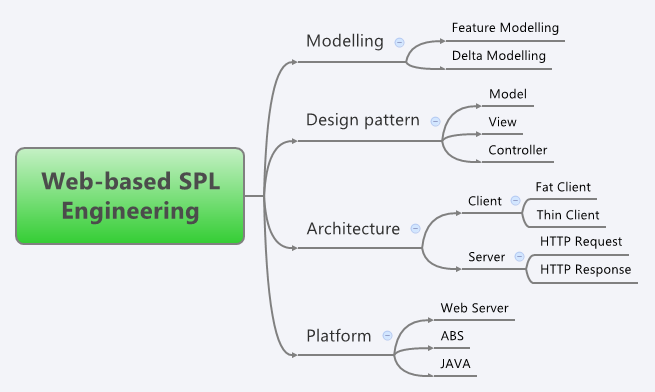
\includegraphics[width=0.8\textwidth]
        {img/kerangka-berpikir.png}
    \caption{Kerangka berpikir}
\end{figure}

\noindent
Setelah penulis mengetahui solusi apa yang harus digunakan agar ABS dapat berjalan di \textit{Application Server}, selanjutnya penulis akan merancang bagaimana pengorganisasian kode yang baik untuk ABS agar sesuai dengan kaidah MVC. Hal ini perlu dilakukan karena nantinya penelitian ini akan menghasilkan sebuah \textit{framework} MVC yang akan digunakan dalam pengembangan SPL berbasis web dengan menggunakan ABS. Dalam hal ini, penulis harus mengkaji terkait peran-peran setiap komponen pada MVC dan kemudian mengimplementasikannya ke ABS. \\

\noindent
Rangkaian proses diatas diharapkan nantinya menghasilkan sebuah framwork MVC yang utuh untuk kemudian diintegrasikan dengan konsep \textit{feature modelling} dan \textit{delta modelling} yang ada di ABS. Hal ini dilakukan agar dapat dihasilkan sebuah framework MVC ABS yang dapat digunakan untuk keperluan pengembangan SPL berbasis web.

%---------------------------------------------------------
\section{Sistematika Penulisan}
%---------------------------------------------------------
berikut adalah sistematika penulisan dari proposal ini:
\begin{itemize}
    \item Bab 1 Pendahuluan \\
    Bab ini berisi tentang latar belakang penelitian, manfaat penelitian, kerangka berpikir, dan sistematika penulisan.
    \item Bab 2 Studi Literatur \\
    Bab ini berisi tentang hasil studi literatur yang dilakukan oleh penulis baik terkait teori-teori dasar yang mendukung penelitian ini ataupun peneletian lain yang masih berkaitan dengan penelitian yang akan dilakukan.
    \item Bab 3 Rumusan Masalah \\
    Bab ini berisi tentang rumusan masalah dari penelitian yang akan dilakukan, ruang lingkup penelitian, serta batasan penelitian.
    \item Bab 4 Rancangan Penelitian \\
    Bab ini berisi tentang rancangan penelitian yang akan dilakukan oleh penulis dan penjelasan dari setiap tahapan-tahapan yang akan dilakukan.
\end{itemize}
\chapter{Metodologi Penelitian}

Berdasarkan rumusan masalah, ruang lingkup penelitian, serta batasan penelitian yang sudah dibahas pada bab sebelumnya, berikut ini adalah metodologi penelitian yang penulis gunakan:

\begin{figure}
    \centering
    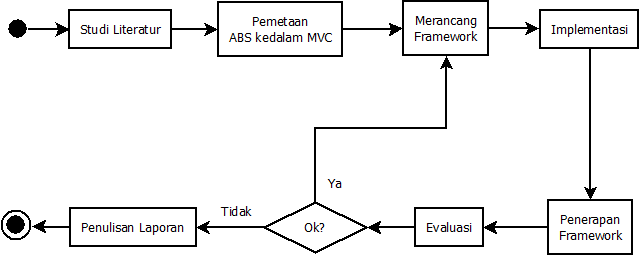
\includegraphics[width=0.8\textwidth]
        {img/metodologi-penelitian.png}
    \caption{Rencana Penelitian}
    \label{fig:metodologiPenelitian}
\end{figure}

Seperti yang terlihat pada Gambar \ref{fig:metodologiPenelitian} diatas, pada awal penelitian penulis melakukan studi literatur untuk mendapatkan pengetahuan terkait teori-teori pendukung yang penulis gunakan dalam melakukan penelitian. Setelah selesai melakukan studi literatur, berikutnya penulis melakukan proses analisa dan pemetaan terhadap bahasa pemodelan ABS untuk kemudian dilakukan pemetaan kedalam komponen-komponen MVC. Seteah proses pemetaan selesai, penulis membuat rancangan ABS MVC Framework sesuai dengan hasil analisa dan pemetaan yang telah dilakukan dan setelah itu penulis melakukan proses implementasi untuk merealisasikan desain yang telah dibuat. Langkah berikutnya adalah melakukan proses penerapan ABS MVC Framework untuk melihat apakah \textit{framework} yang dibuat dapat digunakan untuk membuat sebuah aplikasi berbasis web dan melakukan evaluasi terhadap \textit{framework} tersebut untuk menentukan apakah harus dilakukan perombakan atau sudah layak sebagai sebuah MVC Framework. Berikut ini adalah detail dari setiap tahapan penelitian yang penulis lakukan:

\section{Studi Literatur}

Pada tahap ini penulis melakukan studi literatur dari berbagai sumber seperti buku, artikel ilmian dan web untuk mendapatkan informasi dan pengetahuan terkait teori pendukung yang penulis butuhkan dalam melakukan penelitian ini. Adapun pengetahuan-pengetahuan pendukung yang penulis butuhkan antara lain adalah pengetahuan tentang Hypertext Transfer Protocol (HTTP), pola Model-View-Controller (MVC) dalam pengembangan perangkat lunak, pengetahuan tentang bahasa pemodelan ABS dan pengetahuan tentang \textit{Software Product Line Engineering} (SPLE).

\section{Pemetaan ABS kedalam MVC}

Pada tahap ini penulis melakukan analisa terhadap bahasa pemodelan ABS sesuai dengan pengetahuan yang penulis dapatkan dalam proses studi literatur yang sudah penulis lakukan sebelumnya. Tujuan dari proses analisa yang penulis lakukan ini adalah untuk memetakan bahasa pemodelan ABS kedalam komponen-komponen ABS.

\section{Merancang ABS MVC Framework}

Pada tahap ini penulis membuat rancangan ABS MVC Framework berdasarkan hasil analisa dan pemetaan ABS yang dibuat sebelumnya. Adapun rancangan yang dibuat adalah mengenai bagaimana penyusunan direktori dari \textit{framework} tersebut, bagaiamana karakteristik dari setiap komponen MVC yang dibuat dengan menggunakan ABS serta bagaimana caranya agar komponen MVC yang dibuat dapat menghasilkan sebuah halaman web.

\section{Implementasi}

Pada tahap ini penulis merealisasikan rancangan ABS MVC Framework yang telah penulis buat sebelumnya. Adapun poin-poin implementasi yang dilakukan antara lain adalah mengintegrasikan \textit{framework} ABS yang dibuat dengan JAVA dan \textit{web server} agar \textit{framework} tersebut dapat menghasilkan sebuah halaman web yang utuh.

\section{Penerapan ABS MVC Framework}

Pada tahap ini penulis membuat sebuah aplikasi web dengan menggunakan ABS MVC Framework yang dibuat sekaligus mencoba untuk menerapkan \textit{delta modeling} dan SPLE terhadap \textit{framework} tersebut.

\section{Evaluasi}

Pada tahap ini penulis mengevaluasi hasil penerapan yang dilakukan untuk melihat apakah pelu adanya revisi dan perancangan ulang atau \textit{framework} tersebut sudah sesuai dengan tujuan dari penelitian ini. Apabila hasil evaluasi dari \textit{framework} yang dibuat belum memuaskan, makan akan dilakukan proses revisi rancangan untuk lebih menyempurnakan lagi \textit{framework} yang dibuat. Namun, apabila hasil evaluasi sudah memuaskan maka langkah selanjutnya adalah mendokumentasikan hasil penelitian yang diperoleh kadalam laporan penelitian. Adapun syarat-syarat kelayakan yang penulis tetapkan sebagai parameter keberhasilan dalam proses evaluasi ini antara lain adalah:

\begin{enumerate}
    \item Apakah \textit{framework} yang dihasilkan sudah sesuai dengan kaidah MVC yang berlaku? (sesuai dengan yang ada pada studi literatur)
    \item Apakah \textit{framework} yan dihasilkan dapat diintegrasikan dengan \textit{feature modeling} dan \textit{delta modeling} pada ABS?
    \item Apakah \textit{framework} yang dihasilkan sudah dapat mengasilkan sebuah \textit{complete product} SPL berbasis web? (dapat dijalankan)
\end{enumerate}

\section{Penulisan Laporan}

Pada tahap ini penulis akan menuliskan laporan penelitian dan menarik kesimpulan yang diambil dari penelitian yang sudah dilakukan serta memaparkan temuan-temuan yang diperoleh selama melakukan penelitian.
\chapter{Hasil Studi Literatur}

%---------------------------------------------------------
\section{Model View Controller}
%---------------------------------------------------------
\noindent
\textit{Model-View-Controller} (MVC) atau yang biasa juga dikenal dengan sebutan \textit{Presentation-Abstraction-Control} (PAC) merupakan salah satu pendekatan dalam proses pengembangan perangkat lunak yang ditujukan untuk melakukan pemisahan antara logika aplikasi, data, dan presentasi. Konsep ini dibangun atas kesadaran bahwa sebuah model domain aplikasi yang sama dapat disajikan dan diperlakukan secara berbeda tergantung dari kebutuhan si pengguna aplikasi. Dengan menggunakan pendekatan ini, seorang pengembang perangkat lunak dapat berfokus pada satu bagian saja tanpa harus mengkhawatirkan akan terkena dampak perubahan ataupun memberikan perubahan ke bagian aplikasi lainnya.

\subsection{Sejarah Singkat MVC}
\noindent
Konsep MVC diterapkan pertama kalinya oleh Alan Kay, Dan Ingalls, dan Adele Goldberg pada tahun 1980 ketika mereka merancang bahasa pemrograman smalltalk-80 di Xerox PARC Learning Research Group (LRG) \citep{krasner1988desc}. bahasa pemrograman ini didesain dan dikembangkan dengan menggunakan strategi yang merepresentasikan informasi, tampilan, dan kontrol pada lingkungan pemrogramannya. Strategi ini digunakan dengan tujuan (1) untuk membuat kumpulan komponen sistem spesial yang dibutuhkan dalam mendukung proses pengembangan perangkat lunak yang interaktif serta (2) menyediakan kumpulan komponen sistem umum yang dapat membantu pengembang dalam menciptakan aplikasi grafis yang interaktif dengan mudah \citep{krasner1988desc}. Strategi dan tujuan tersebut dibuat dalam rangka menjawab isu utama dalam pengembangan perangkat lunak yaitu terkait pemanfaatan kembali komponen yang telah dibuat (\textit{reusability}) dan kemudahan dalam menggabungkan setiap komponen aplikasi (\textit{plugability}). \\

\noindent
Belajar dari pengalamannya dalam mengembangkan smalltalk-76, para pengembang smalltalk-80 menemukan bahwa untuk mencapai sebuah modularitas yang tinggi diperlukan adanya tiga buah pemisahan fokus dalam pengembangan aplikasi. Tiga buah pemisahan fokus tersebut antara lain adalah (1) memisahkan setiap komponen yang merepresentasikan model domain aplikasi dengan (2) cara yang digunakan untuk merepresentasikan model tersebut ke pengguna aplikasi dan (3) cara yang digunakan oleh pengguna dalam berinteraksi dengan model tersebut. Tiga buah pemisahan tersebut dapat terangkum dalam sebuah konsep yang disebut dengan \textit{Model-View-Controller} (MVC).

\subsection{Penerapan MVC dalam Pengembangan Aplikasi Web}
Aplikasi web merupakan aplikasi yang tergolong interaktif karena aplikasi jenis ini banyak memiliki elemen-elemen yang dapat digunakan untuk berinteraksi dengan penggunannya. Sebagai contoh, dalam sebuah halaman situs web tentunya kita akan menemukan banyak tombol, gambar, tautan, dan kotak isian yang dapat kita gunakan untuk berinteraksi dengan situs web tersebut. Untuk sebuah aplikasi yang tergolong interaktif, adanya pemisahan antara logika aplikasi, data, dan presentasi tentunya akan dapat meningkatkan fleksibilitas aplikasi tersebut dari segi pengembangan. \\

\noindent
Pada dasarnya, arsitektur apliksi berbasis web terbagi menjadi dua bagian yaitu \textit{client} dan \textit{server}. Dengan arsitektur yang seperti ini, para pengembang aplikasi tidak dapat menentukan dengan jelas bagaimana bentuk partisi yang harus dibuat untuk aplikasi tersebut. Sebagai contoh, dengan adanya pembagian antara \textit{client} dan \textit{server}, para pengembang aplikasi harus menentukan dimanakah komponen \textit{view} akan dibentuk? Apakah komponen ini akan dibentuk di tingkat \textit{client} ataukah di tingkat \textit{server}. Begitupun dengan komponen \textit{Model} dan \textit{Controller
}-nya. Apakah komponen-komponen tersebut akan akan dibuat di tingkat \textit{client}, \textit{server}, atau keduanya? Pada akhirnya, keputusan dalam menentukan skema partisi yang dipakai akan sangat bergantung pada teknologi yang digunakan \citep{leff2001web}. \\

\noindent
Permasalahan terkait pemisahan antara \textit{client} dan \textit{server} pada aplikasi berbasis web menjadikan penerapan MVC lebih sulit. Proses penerapan MVC akan dapat berhasil apabila (1) para pengembang aplikasi sudah mengetahui bagaimana skema partisi yang akan diterapkan serta (2) teknologi dan infrastruktur yang ada \textit{compatible} dengan skema partisi yang diterapkan. Oleh karena itu, perlu adanya sebuah pendekatan yang dapat digunakan oleh para pengembang untuk memastikan dua hal tersebut.

%---------------------------------------------------------
\section{Software Product Line Engineering (SPLE)}
%---------------------------------------------------------
\noindent
\textit{Software Product Line Engineering} (SPLE) merupakan sebuah paradigma yang digunakan dalam proses pengembangan perangkat lunak dengan menggunakan prinsip \textit{platform} dan \textit{mass customisation} \citep[p.~14]{pohl2005software}. Dalam industri perangkat lunak, istilah \textit{platform} atau \textit{software platform} biasa diartikan sebagai sebuah sistem komputer (misal: prosesor atau kombinasi antara perangkat keras dengan sistem operasi) yang menyebabkan dapat berjalannya sebuah program komputer. Sedangkan dalam konteks SPLE, yang dimaksud dengan \textit{platform} adalah sebuah subsistem dan \textit{interface} yang membentuk sebuah struktur umum dimana nantinya sebuah produk turunan dapat dikembangkan dan diproduksi secara efisien \citep[p.~15]{pohl2005software}. \\

\noindent
Dalam paradigma SPLE, proses pengembangan perangkat lunak dibagi menjadi dua bagian yaitu \textit{Domain Engineering} dan \textit{Application Engineering} \citep[p.~21]{pohl2005software}. \textit{Domain Engineering} adalah sebuah proses dalam SPLE dimana pada tahap ini seluruh \textit{commonality} dan \textit{variability} dari SPL didefinisikan dan direalisikan. Sedangkan tahap \textit{Application Engineering} adalah sebuah proses dimana aplikasi dari SPL dibuat dengan cara memanfaatkan \textit{domain artifact} yang telah dibuat pada tahap sebelumnya dan mengeksploitasi \textit{variability} yang ada di dalam SPL tersebut. Tahapan-tahapan proses dalam SPLE ini biasa disebut dengan istilah \textit{SPLE Framework}. \\

\begin{figure}
    \centering
    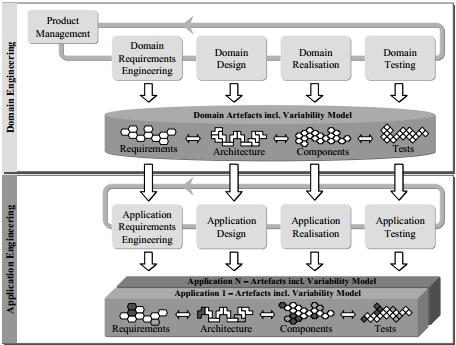
\includegraphics[width=0.8\textwidth]
        {img/sple-process.png}
    \caption{SPLE Framework}
\end{figure}
\vspace{-0.8cm}
\begin{center}
{\small Sumber gambar: \citep{pohl2005software}}
\end{center}

%---------------------------------------------------------
\section{Abstract Behavioural Spesification (ABS)}
%---------------------------------------------------------
\noindent
Abstract Behavioural Specification Language (ABS) merupakan sebuah bahasa pemodelan yang dibuat oleh konsorsium uni eropa di bawah proyek bernama \textit{Highly Adaptable and Trustworthy Software using Formal Method} (HATS). Tujuan dari proyek HATS dalam menciptakan ABS adalah untuk menciptakan sebuah pendekatan yang \textit{model-centric} dalam melakukan proses perancangan, implementasi dan verifikasi dari sebuah sistem yang \textit{highly-configurable} \citep{clarke2012variability}. Pada dasarnya ABS dibagi kedalam beberapa layer (lihat gambar 2.x) yang diantaranya adalah \textit{functional abstraction}, \textit{OO-Imperative layer}, \textit{Concurency Model} dan \textit{ABS Core}. \\

\begin{figure}
    \centering
    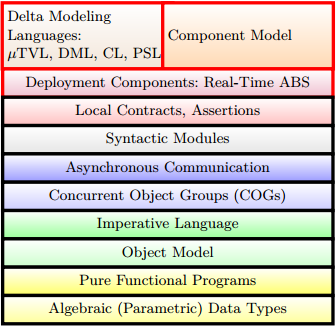
\includegraphics[width=0.6\textwidth]
        {img/abs-layers.png}
    \caption{ABS Layer}
\end{figure}
\vspace{-0.8cm}
\begin{center}
{\small Sumber gambar: \citep{hahnle2013hats}}
\end{center}

\noindent
Sebagai sebuah bahasa pemrograman \textit{imperative} yang menganut konsep \textit{Object Oriented}, secara umum ABS memiliki sintaks yang sama dengan bahasa pemrograman JAVA (walaupun lebih sederhana). Salah satu perbedaan yang paling mendasar antara ABS dengan JAVA adalah pada konsep \textit{code reuse}-nya. Pada bahasa pemrograman JAVA, konsep \textit{code reuse} diimplementasikan dengan cara membuat \textit{code inheritance} sedangkan pada ABS konsep tersebut diimplementasikan dalam betuk \textit{code deltas} \citep{hahnle2013hats}. \textit{code deltas} pada ABS merupakan sebuah kumpulan kode yang mendeskripsikan perubahan-perubahan kode pada kelas yang dituju. Dengan adanya konsep ini, ABS dapat melakukan manipulasi kelas seperti menambah atau menghilangkan \textit{variable} dan \textit{method}. \\

\noindent
Seperti yang sudah disebutkan sebelumnya bahwa di dalam ABS konsep \textit{code reuse} diimplementasikan dalam bentuk \textit{code deltas}. \textit{Code deltas} tersebut nantinya akan digunakan untuk memodelkan \textit{variability} yang terjadi di tingkat \textit{source code}. pemodelan \textit{variability} ini merupakan sebuah pendekatan yang dilakukan oleh ABS dalam membangun sebuah SPL. Proses pemodelan \textit{variability} ini biasa disebut juga sebagai proses \textit{Delta Modelling}. \\

\noindent
\textit{Delta Modelling} merupakan sebuah pendekatan yang fleksible dan modular dalam mewujudkan berbagai macam variasi produk dengan menggunakan kembali artifak-artifak yang ada \citep{hahnle2013hats}. Dalam proses \textit{Delta Modelling}, realisasi dari SPL dibentuk dari dua bagian yaitu \textit{core module} dan \textit{delta module}. \textit{Delta module} berisi fungsi-fungsi yang berlaku umum terhadap semua varian produk yang akan dibuat sedangkan \textit{delta modul} merupakan enkapsulasi dari perubahan-perubahan yang akan terjadi pada \textit{core product} untuk kemudian menghasilkan varian produk yang lain. \\

\begin{figure}
    \centering
    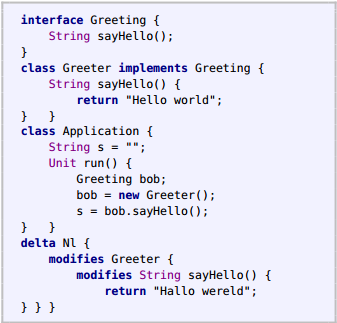
\includegraphics[width=0.6\textwidth]
        {img/delta-modelling-1.png}
\end{figure}

\begin{figure}
    \centering
    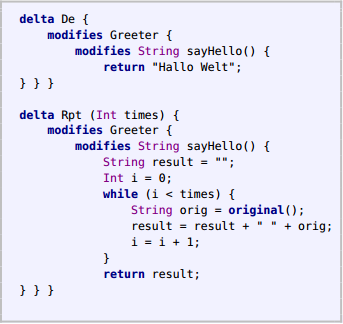
\includegraphics[width=0.6\textwidth]
        {img/delta-modelling-2.png}
    \caption{Delta Modelling pada ABS}
\end{figure}\vspace{-0.8cm}
\begin{center}
{\small Sumber gambar: \citep{clarke2012variability}}
\end{center}
\chapter{Perancangan ABS MVC Framework}

Bab ini membahas tentang rancangan ABS MVC Framework yang penulis buat sebelum melakukan tahap implementasi kode.

\section{Gambaran Umum}

ABS MVC Framework merupakan sebuah alat bantu yang dapat digunakan oleh para pengembang perangkat lunak dalam membuat sebuah aplikasi berbasis web dengan menggunakan bahasa pemodelan ABS. Layaknya MVC Framework yang lain seperti Play Framework (JAVA) \footnote{https://www.playframework.com/}, Laravel (PHP) \footnote{http://laravel.com/} dan Code Igniter (PHP) \footnote{https://github.com/bcit-ci/CodeIgniter}, ABS MVC Framework dibuat dengan tujuan untuk membantu para pengembang perangkat lunak dalam menerapkan pola Model-View-Controller (MVC) untuk keperluan pengembangan aplikasi web. Oleh karena itu, terdapat beberapa fitur utama yang harus dimiliki oleh ABS MVC Framework sebagai sebuah MVC Framework yang diantara adalah:

\begin{enumerate}
    \item ABS MVC Framework harus dapat membantu pengguna \textit{framework} untuk dapat menghasilkan sebuah halaman web yang statis maupun dinamis.
    \item ABS MVC Framework harus dapat membantu pengguna \textit{framework} untuk dapat memisahkan kode yang mereka buat kedalam komponen Model, View dan Controller.
    \item Setiap komponen MVC yang dibuat harus memiliki karakteristik yang jelas sehingga dapat dibedakan mana komponen Model, View dan Controller.
    \item ABS MVC Framework harus dapat membantu pengguna \textit{framework} dalam memetakan setiap HTTP \textit{request} yang diterima kedalam setiap operasi yang spesifik sehingga diperoleh sebuah halaman web yang sesuai.
    \item ABS MVC Framework harus dapat membantu pengguna \textit{framework} dalam menerima dan memproses \textit{input} yang diberikan oleh pengguna aplikasi web dalam bentuk HTTP POST atau GET data. 
\end{enumerate}

Berdasarkan rincian fitur di atas, penulis membuat sebuah rancangan untuk ABS MVC Framework yang nantinya akan dijadikan acuan dalam proses implementasi.

\section{Rancangan ABS MVC Framework}

Setelah adanya pemaparan tentang gambaran umum fitur yang harus dimiliki oleh ABS MVC Framework, penulis membuat sebuah desain tentang bagaimana alur kerja ABS MVC Framework dimulai dari mendapatkan HTTP \textit{request} sampai dengan menampilkan halaman web pada \textit{web browser}. Berikut ini adalah desain yang penulis buat untuk ABS MVC Framework:

\begin{figure}
    \centering
    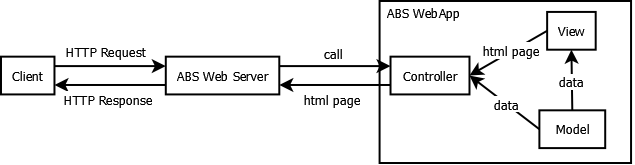
\includegraphics[width=0.8\textwidth]{img/abs-mvc.png}
    \caption{Rancangan ABS MVC Framework}
    \label{fig:mvcFrameworkDesign}
\end{figure}

Seperti yang terlihat pada Gambar \ref{fig:mvcFrameworkDesign} di atas, alur pembuatan halaman web dimulai dari sebuah HTTP \textit{request} yang dikirimkan oleh pengguna web kepada \textit{web server} melalui aplikasi \textit{web browser} yang mereka gunakan. Setelah HTTP \textit{request} tersebut diterima oleh \textit{web server}, berikutnya adalah meneruskan \textit{request} tersebut kapada ABS MVC Framework untuk memperoleh halaman web yang diinginkan. Setelah \textit{web server} berhasil memperoleh halaman web yang diinginkan, selanjutnya \textit{web server} akan memberikan halaman tersebut kepada \textit{web browser} untuk kemudian ditampilkan kepada pengguna web. Melalui mekanisme inilah seorang pengguna web dapat mengakses halaman web yang telah dibuat.\\

Berdasarkan pada rancangan tersebut, penulis menyimpulkan bahwa terdapat tiga buah isu yang harus diperhatikan dalam menyusun ABS MVC Framework yang diantaranya adalah:

\begin{enumerate}
    \item Bagaimana mekanisme pemetaan yang dapat dilakukan dalam memetakan setiap HTTP \textit{request} kedalam setiap komponen Controller pada ABS MVC Framework.
    \item Bagaimana mekanisme yang dapat dilakukan agar ABS MVC Framework dapat menerima dan memproses setiap HTTP POST dan GET data yang diterima oleh \textit{web server}.
    \item Bagaimana karakteristik setiap komponen MVC yang ada di pada ABS MVC Framework.
\end{enumerate}

\subsection{Mekanisme Pemetaan HTTP Request}

Dalam konteks pengembangan aplikasi web dengan menggunakan MVC Framework, setiap \textit{request} yang diberikan oleh pengguna aplikasi harus dipetakan kedalam setiap komponen Controller yang dibuat. Tujuannya adalah agar \textit{web server} dapat mengetahui dengan pasti komponen Controller manakah yang harus dipanggil pada saat menerima \textit{request} dari \textit{web browser}. Untuk dapat merealisasikan hal tersebut, dibutuhkan adanya mekanisme khusus yang dapat digunakan oleh pengguna \textit{framework} untuk dapat memetakan setiap \textit{request} yang diterima secara cepat dan mudah.

\begin{figure}
    \centering
    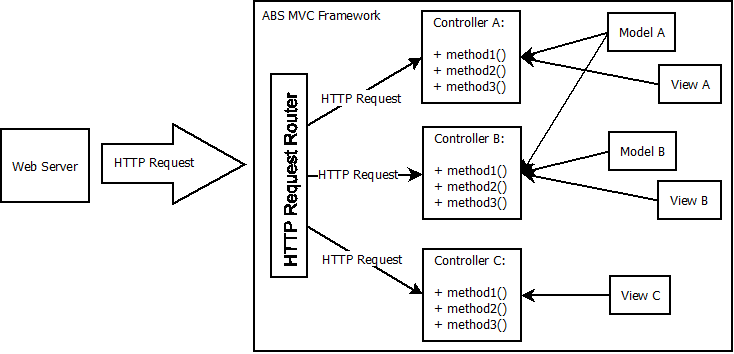
\includegraphics[width=0.8\textwidth]{img/mvc-routing-mechanism}
    \caption{Rancangan mekanisme pemetaan \textit{request} pada ABS MVC Framework}
    \label{fig:mvcRoutingMechanism}
\end{figure}

Seperti yang terlihat pada Gambar \ref{fig:mvcFrameworkDesign} di atas, pada ABS MVC Framework proses pemetaan HTTP \textit{request} dilakukan oleh sebuah komponen yang bernama HTTP Request Router. Melalui komponen ini, setiap \textit{request} yang diberikan oleh \textit{web server} akan dipetakan kedalam setiap komponen Controller yang berada di dalam \textit{framework}. Dengan demikian, ABS MVC Framework akan dapat menghasilkan halaman web yang sesuai dengan permintaan dari \textit{web browser}.

\subsection{Mekanisme Penanganan HTTP POST dan GET data}

Seperti yang sudah penulis sebutkan pada rincian fitur ABS MVC Framework, salah satu fitur yang harus dimiliki oleh \textit{framework} ini selain dapat melakukan pemetaan HTTP Request kedalam komponen Controller adalah kemampuannya dalam menerima dan memperoses \textit{input} yang diberikan dalam bentuk HTTP POST dan GET data. Tujuan dari adanya fitur ini adalah agar aplikasi web yang dibuat dapat menerima \textit{input} dari pengguna dan menghasilkan sebuah halaman web yang dinamis. Untuk dapat merealisasikan hal tersebut, dibutuhkan adanya sebuah mekanisme yang dapat digunakan oleh \textit{web server} untuk dapat meneruskan HTTP POST dan GET data yang diterima dari \textit{web server} kepada ABS MVC Framework. Berikut ini adalah rancangan yang penulis buat untuk mengani HTTP POST dan GET data pada ABS MVC Framework.

\begin{figure}
    \centering
    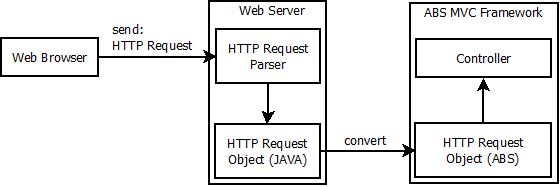
\includegraphics[width=0.8\textwidth]{img/mvc-http-input.png}
    \caption{Rancangan mekanisme penanganan \textit{input} pada ABS MVC Framework}
    \label{fig:mvcHttpInputMechanism}
\end{figure}

Terlihat pada Gambar \ref{fig:mvcHttpInputMechanism} di atas, setiap HTTP \textit{request} yang diterima oleh \textit{web server} akan dibuat menjadi sebuah objek JAVA. Objek yang berisikan HTTP POST atau GET data ini nantinya akan dikonversi menjadi sebuah Objek ABS dan diberikan kepada ABS MVC Framework untuk kemudian digunakan oleh komponen Controller. Dengan menggunakan cara ini, pengguna ABS MVC Framework dapat menerima dan memproses \textit{input} yang diberikan oleh \textit{web server} melalui komponen Controller yang dibuat.

\subsection{Karakteristik komponen MVC pada ABS MVC Framework}

Salah satu tujuan dari penggunaan MVC Framework dalam proses pengembangan perangkat lunak adalah untuk membantu para pengembang dalam memecah kode program yang dibuat kedalam komponen Model, View dan Controller. Untuk dapat memecah kode program kedalam tiga buah komponen tersebut, perlu adanya karakteristik yang jelas yang dapat membedakan ketiga buah komponen tersebut. Oleh karena itu, penulis perlu mendefinisikan karakteristik dari setiap komponen MVC yang ada di dalam ABS MVC Framework untuk mempermudah para pengembang dalam mengelompokan kode program yang mereka buat.\\

Berikut ini adalah karakteristik yang sudah penulis rancang untuk setiap komponen MVC pada ABS MVC Framework:

\begin{itemize}
    \item \textbf{Model}: Komponen ini merupakan komponen yang merepresentasikan data pada aplikasi yang dibuat. Dalam membuat komponen Model ini, diharapkan komponen ini dibentuk sesederhana mungkin dengan hanya berisikan atribut-atribut yang berkaitan dengan data beserta \textit{method} aksesor dan mutatornya. Setiap kode yang mengandung proses bisnis aplikasi tidak boleh diletakan di dalam komponen ini.
    \item \textbf{View}: Komponen ini berperan dalam mempresentasikan data yang berasa dari komponen Model kepada pengguna aplikasi dalam bentuk halaman web. Dalam konteks pengembangan aplikasi web, diharapkan komponen ini dapat didefinisikan dengan menggunakan sintaks HTML untuk memudahkan para pengembang dalam proses pembuatannya. Selain itu, dikarenakan komponen ini ditujukan untuk menampilkan komponen Model yang diberikan, maka komponen ini harus bisa mengakses komponen Model secara langsung.
    \item \textbf{Controller}: Komponen ini merupakan komponen yang berisikan proses bisnis dari aplikasi web yang dibuat. Pada komponen inilah pengembang perangkat lunak akan memproses setiap \textit{input} yang diberikan oleh pengguna aplikasi dan mengintegrasikannya dengan komponen Model dan View dalam menghasilkan sebuah halaman web yang utuh. Komponen ini merupakan komponen utama dalam sebuah aplikasi web berbasis MVC dan oleh karenanya, keberadaan komponen ini tidak dapat dihilangkan dari dalam aplikasi web yang dibuat.
\end{itemize}

Sampai pada tahap ini, penulis telah berhasil membuat rancangan untuk ABS MVC Framework. Langkah berikutnya adalah melakukan proses implementasi (\textit{coding}) untuk dapat merealisasikan rancangan yan dibuat.

\chapter{Implementasi}
Bab ini memaparkan secara kronologis tentang proses eksperimen yang telah dilakukan oleh penulis.

\section{Mengintegrasikan ABS dengan JAVA}
Berdasarkan hasil studi literatur yang telah dilakukan, penulis mengetahui bahwa salah satu fitur yang dimiliki oleh ABS adalah kemampuannya untuk dapat di\textit{compile} kedalam bahasa JAVA sehingga nantinya kode ABS tersebut dapat dijalankan di dalam JAVA Runtime Environment (JRE). Berdasarkan informasi tersebut, penulis menarik kesimpulan bahwa jika penulis membuat sebuah JAVA class yang dibuat secara \textit{native}, maka JAVA Class tersebut akan dapat memanggil class ABS yang sudah di\textit{compile} menjadi JAVA Class juga.\\

Sebelum penulis mencoba untuk mengintegrasikan secara langsung ABS dengan JAVA, penulis mencoba untuk mengetahui hasil kompilasi kode ABS yang diubah kedalam JAVA. berikut adalah kode ABS sederhana yang penulis buat beserta hasil kompilasinya ke dalam kode JAVA.

\begin{lstlisting}[
caption=Kode ABS beserta Main Blocknya,
label={lst:absSederhana},
escapeinside={@}{@}
]
module UserModule;

interface User
{
	String getUsername();
}

class UserImpl implements User
{
	String getUsername() @\label{lst:absString}@
	{
		return "salman"; @\label{lst:absString2}@
	}
}

//ABS Main block
{
	User myUser = new local UserImpl(); @\label{lst:absCreateObject}@
	String username = myUser.getUsername();
}
\end{lstlisting}

\begin{lstlisting}[ 
firstnumber=64,
caption=Hasil kompilasi ABS ke JAVA untuk method getUsername(),
label={lst:absjavaGetUsername},
escapeinside={@}{@},
]
// User.abs:10:2: 
public final abs.backend.java.lib.types.ABSString getUsername() {
    ...
    return abs.backend.java.lib.types.ABSString.fromString("salman"); @\label{lst:absjavaString}@
}
\end{lstlisting}

\begin{lstlisting}[
caption=Hasil kompilasi ABS ke JAVA untuk Main Block,
label={lst:absjavaMainBlock},
escapeinside={@}{@}
]
package UserModule;
public class Main extends abs.backend.java.lib.runtime.ABSObject {
    public static void main(java.lang.String[] args) throws Exception {
        abs.backend.java.lib.runtime.StartUp.startup(args,Main.class);
    }
    public java.lang.String getClassName() { return "Main"; }
    public java.util.List<java.lang.String> getFieldNames() { return java.util.Collections.EMPTY_LIST; }
    public Main(abs.backend.java.lib.runtime.COG cog) { super(cog); }
    public abs.backend.java.lib.types.ABSUnit run() {
         {
            ...
            UserModule.User_i myUser = UserModule.UserImpl_c.__ABS_createNewObject(this); @\label{lst:absjavaCreateObject}@
            
            ...
            abs.backend.java.lib.types.ABSString username = abs.backend.java.lib.runtime.ABSRuntime.checkForNull(myUser).getUsername();
            if (__ABS_getRuntime().debuggingEnabled()) __ABS_getRuntime().getCurrentTask().setLocalVariable("username",username);
        }
        
        return abs.backend.java.lib.types.ABSUnit.UNIT;
    }
}
\end{lstlisting}

Seperti yang terlihat pada kode \ref{lst:absjavaMainBlock} baris \ref{lst:absjavaCreateObject}, terdapat perbedaan pada kode JAVA hasil kompilasi dari ABS dalam membuat \textit{instance} dari sebuah objek. Dalam bahasa JAVA yang standar, untuk dapat membuat \textit{instance} dari sebuah class adalah dengan menggunakan kata kunci \texttt{new} seperti misalnya \texttt{new UserImpl()}. Sedangkan pada kode JAVA hasil kompilasi ABS menggunakan kata kunci \texttt{\_\_ABS\_createNewObject(this)} yang diakses secara \textit{static}.\\

Berdasarkan hasil percobaan tersebut penulis mengetahui bahwa sintaks ABS yang terdapat pada kode \ref{lst:absSederhana} baris \ref{lst:absCreateObject} adalah \textit{equivalent} dengan sintaks JAVA yang terdapat pada kode \ref{lst:absjavaMainBlock} baris \ref{lst:absjavaCreateObject}. Dengan demikian, penulis dapat menyimpulkan bahwa ketika penulis ingin mencoba untuk memanggil class JAVA hasil kompilasi ABS dari class JAVA yang \textit{native} maka penulis harus melakukan pemanggilan fungsi seperti yang terlihat pada kode kode \ref{lst:absjavaMainBlock} baris \ref{lst:absjavaCreateObject} tersebut.\\

Selain terdapat perbedaan dalam cara membuat \textit{instance} dari sebuah class, terdapat pula perbedaan pada tipe data yang digunakan oleh JAVA hasil kompilasi dari ABS dengan JAVA yang \textit{native}. Jika kita melihat kode \ref{lst:absSederhana} baris \ref{lst:absString} dan \ref{lst:absString2} penulis menggunakan sebuah tipe data \texttt{String} seperti layaknya tipe data \texttt{String} pada JAVA. Akan tetapi ketika kode ABS tersebut di\textit{compile} kedalam bahasa JAVA, ternyata tipe data \texttt{String} tersebut diubah menjadi \texttt{ABSString} seperti yang terlihat pada kode \ref{lst:absjavaGetUsername} baris \ref{lst:absjavaString}. Berdasarkan hasil percobaan tersebut penulis berkesimpulan bahwa ketika penulis ingin mengintegrasikan ABS dengan JAVA, penulis perlu melakukan konversi tipe data dari tipe data milik JAVA ABS menjadi tipe data standar JAVA.\\

Kesimpulan yang penulis dapatkan setelah melakukan percobaan ini adalah: (1) bahwa untuk dapat membuat sebuah \textit{instance} dari class JAVA hasil kompilasi ABS tidak dapat dilakukan dengan menggunakan kata kunci \texttt{new} seperti pada JAVA yang \textit{native} dan (2) terdapat perbedaan tipe data antara \textit{native} JAVA dengan JAVA hasil kompilasi ABS sehingga perlu adanya penyesuaian lebih lanjut agar penulis dapat mengintegrasikan ABS dengan \textit{native} JAVA.

\section{Membuat halaman web sederhana menggunakan ABS}
Setelah penulis melakukan percobaan sederhana untuk mengetahui cara mengintegrasikan ABS dengan JAVA, selanjutnya penulis melakukan percobaan untuk dapat membuat halaman web sederhana dengan menggunakan ABS. Seperti yang telah kita ketahui bersama, untuk dapat menampilkan sebuah halaman web pada web browser, dibutuhkan adanya sebuah web server yang nantinya akan dapat melayani permintaan dari web browser. Dalam percobaan ini penulis membuat sebuah web server sederhana dengan menggunakan \texttt{ServerSocket} pada JAVA untuk membuka \textit{port} dan menerima \textit{request} dari \textit{web browser} yang nantinya akan memanggil class JAVA hasil kompilasi ABS untuk mendapatkan halaman web yang diinginkan (lihat gambar \ref{fig:howAbsGenerateHTML}).

\begin{figure}
    \centering
    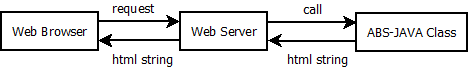
\includegraphics[
        width=0.8\textwidth
    ]{img/request-webserver-abs.png}
    \caption{Bagaimana web server menghasilkan sebuah halaman web}
    \label{fig:howAbsGenerateHTML}
\end{figure}

Untuk dapat mensimulasikan proses seperti yang telah digambarkan pada gambar \ref{fig:howAbsGenerateHTML} di atas, pertama-tama penulis membuat sebuah ABS Module yang fungsinya adalah untuk dapat menghasilkan sebuah halaman sederhana dan memberikannya kepada \textit{web server}. berikut adalah kode ABS yang penulis buat untuk menghasilkan sebuah halaman web:

\begin{lstlisting}[
caption=Kode ABS untuk menghasilkan halaman HTML,
label={lst:absWelcomeView},
]
module ABS.MVC.View.WelcomeView;

interface WelcomeView
{
	String generateView();
}

class WelcomeViewImpl implements WelcomeView
{
	
	String generateView() {		
		String html = "<!DOCTYPE HTML>";
		html = html + "<html>";
		html = html + "<body>";
		html = html + "<h1>Welcome!!</h1>";
		html = html + "Please login <a href='/login.abs'>here</a>";
		html = html + "<br />";
		html = html + "<p>This page was generated from ABS Class</p>";
		html = html + "</body>";
		html = html + "</html>";
		
		return html;
	}
}
\end{lstlisting}

Seperti yang terlihat pada kode \ref{lst:absWelcomeView} di atas, penulis menggunakan \texttt{String} berisikan kode HTML yang disambung-sambung (\textit{concatted String}) untuk menghasilkan sebuah halaman web. Rencananya adalah string yang sudah dihasilkan oleh halaman ABS Module ini nantinya akan diberikan ke \textit{web server} untuk kemudian diberikan ke \textit{web browser} dan ditampilkan ke \textit{user}. Sebagai awalan, penulis membuat sebuah class JAVA yang ditujukan untuk memanggil class JAVA hasil kompilasi ABS tersbut untuk kemudian ditampilkan di \textit{console} dengan menggunakan \texttt{System.out.println()}. Berikut adalah kode JAVA yang dibuat oleh penulis beserta hasil pemanggilan class ABS-nya.

\begin{lstlisting}[
caption=Kode JAVA untuk memanggil ABS,
label={lst:javaCallABS},
escapeinside={@}{@}
]
package com.fmse.absserver;

public class ABSMain extends ABSObject 
{
    ...
       
    public ABSUnit run() {
        System.out.println("ABSMain running..");
        WelcomeView_i view = WelcomeViewImpl_c.__ABS_createNewObject(this); @\label{lst:javaCreateABSObject}@
        ABSString html = ABSRuntime.checkForNull(view).generateView(); @\label{lst:javaCallABSMethod}@
        System.out.println(html.getString());
        return ABSUnit.UNIT; 
    }
    
    public static void main(String[] args) throws Exception {
        StartUp.startup(new String[0], ABSMain.class);
    }
}
\end{lstlisting}

\begin{figure}
    \centering
    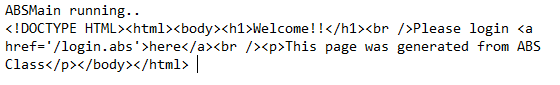
\includegraphics[
        width=0.8\textwidth
    ]{img/java-call-abs-result.png}
    \caption{Hasil dari pemanggilan ABS yang berisikan HTML String}
    \label{fig:javaABSCallResult}
\end{figure}

Terlihat pada kode \ref{lst:javaCallABS} baris \ref{lst:javaCreateABSObject} dan \ref{lst:javaCallABSMethod} di atas, penulis membuat sebuah \textit{instance} dari class \texttt{WelcomView} serta melakukan pemanggilan fungsi \texttt{generateView()} untuk mendapatkan \texttt{String} HTML yang telah dibuat. Hasil dari pemanggilan fungsi \texttt{generateView()} pada class \texttt{WelcomeView} tersebut adalah sebuah \texttt{String} panjang berisikan kode HTML seperti yang terlihat pada gambar \ref{fig:javaABSCallResult}.\\

Setelah penulis berhasil memanggil class JAVA hasil kompilasi ABS untuk mendapatkan HTML String, langkah selanjutnya adalah memberikan HTML String tersebut kepada web browser. Untuk dapat melakukan hal tersebut, penulis akan membuat sebuah web server sederhana dengan menggunakan class \texttt{ServerSocket} pada JAVA. Berikut adalah kode JAVA yang penulis buat untuk dapat menerima request dari \textit{web browser} dan memberikan halaman web yang diinginkan kepada \textit{web browser}.

\begin{lstlisting}[
caption=Potongan kode web server yang memanggil class ABS,
label={lst:javaSimpleWebServer},
escapeinside={@}{@}
]
public class ABSHttpServer extends ABSObject {

    ...
    
    public ABSUnit run() {
        try {
            ServerSocket serverSocket = new ServerSocket(8080); @\label{lst:javaCreateSocket}@
            while(true) {
                Socket remote = serverSocket.accept(); @\label{lst:javaCreateSocket2}@
                BufferedReader in = new BufferedReader(
                        new InputStreamReader(remote.getInputStream()));
                String request = in.readLine();
                String[] protocols = request.split(" ");
                
                ...
                
                if(protocols[1].equals("/")) { @\label{lst:serverStartCallABS}@
                	WelcomeView_i view = WelcomeViewImpl_c.__ABS_createNewObject(this); 
                    html = ABSRuntime.checkForNull(view).generateView().getString();
                    out.println(html);
                } @\label{lst:serverEndCallABS}@
                
                out.flush();
                remote.close();
            }
        }
        catch(Exception e) {
            e.printStackTrace();
        }
        
        return ABSUnit.UNIT;
    }
    
    ...
}
\end{lstlisting}

Pada kode \ref{lst:javaSimpleWebServer} baris \ref{lst:javaCreateSocket} dan \ref{lst:javaCreateSocket2} di atas, terlihat bahwa penulis melakukan pembuatan \texttt{ServerSocket} dan membuka \textit{port} 8080 untuk menerima \textit{request} dari \textit{web browser}. Setelah \textit{web server} menerima \textit{request} dari \textit{web browser}, berikutnya \textit{web server} akan mencocokan URL yang diberikan oleh \textit{web browser} seperti yang terlihat pada gambar \ref{fig:webBrowserRequest}. Apabila URL yang diminta cocok dengan salah satu kondisi yang ada di \textit{web server}, berikutnya \textit{web server} akan melakukan pemanggilan class ABS seperti yang terlihat pada kode \ref{lst:javaSimpleWebServer} baris \ref{lst:serverStartCallABS} - \ref{lst:serverEndCallABS}. Setelah HTML String berhasil diterima oleh \textit{web server} berikutnya akan diberikan ke \textit{web browser} melalui \texttt{OutputStream} pada \texttt{ServerSocket} untuk kemudian ditampilkan di \textit{web browser} seperti yang terlihat pada gambar di bawah ini.

\begin{figure}
    \centering
    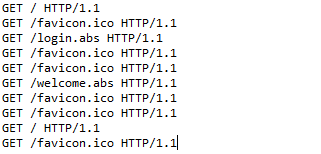
\includegraphics[
        width=0.6\textwidth
    ]{img/web-browser-request.png}
    \caption{Contoh \textit{request} dari \textit{web browser}}
    \label{fig:webBrowserRequest}
\end{figure}

\begin{figure}
    \centering
    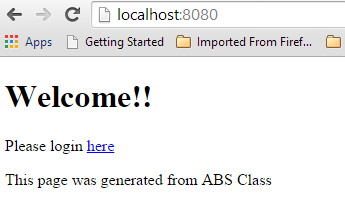
\includegraphics[
        width=0.6\textwidth
    ]{img/abs-welcome-view.png}
    \caption{Halaman web yang dibuat menggunakan ABS}
    \label{fig:javaABSCallResult}
\end{figure}

Sampai pada tahap ini penulis telah berhasil membuat sebuah halaman web sederhana dengan menggunakan ABS. Langkah berikutnya yang penulis lakukan adalah mencoba untuk memetakan ABS kedalam komponen-komponen MVC untuk membuat sebuah MVC Framework.

\section{Memetakan ABS kedalam komponen MVC}
Salah satu tujuan dibentuknya framework MVC untuk ABS adalah agar para pengembang perangkat lunak dapat dengan mudah memisahkan kode program yang mengandung logika bisnis, data dan presentasi dari sebuah aplikasi. Oleh karena itu, sebelum membentuk sebuah framework MVC secara utuh, penulis perlu melakukan pemetaan terhadap kode ABS kedalam setiap komponen Model, View dan Controller (MVC). Tujuan dari dilakukannya proses pemetaan ini adalah agar penulis mendapatkan gambaran bagaimana seharusnya komponen Model, View dan Controller tersebut dibuat dengan menggunakan ABS.\\

Secara umum ABS memiliki sintaks yang tidak jauh berbeda dengan JAVA. Selain itu ABS juga sudah mendukung model pemrograman Object-Oriented Programming (OOP). Oleh karenanya penulis dapat menggunakan pengalaman penulis dalam menggunakan framework MVC untuk JAVA dan PHP (karena keduanya memiliki konsep OOP) beserta hasil studi literatur yang sudah penulis lakukan dalam melakukan proses pemetaan ini. Jika kita merujuk pada publikasi yang dibuat oleh \cite{krasner1988desc} dan \cite{leff2001web} tentang MVC, berikut adalah karakteristik dari masing-masing komponen MVC:

\begin{itemize}
    \item Model: merupakan bagian dari aplikasi yang merepresentasikan data pada aplikasi dan memiliki fungsi yang dapat digunakan untuk memanipulasi data sesuai dengan input yang diberikan.
    \item View: merupakan bagian dari aplikasi yang berfungsi untuk menampilkan informasi kepada user baik dalam bentuk teks ataupun grafis.
    \item Controller: merupakan bagian dari aplikasi yang berfungsi untuk menerima, mengintepretasikan dan memproses setiap \textit{input} yang diberikan oleh \textit{user}.
\end{itemize}

Berdasarkan karakteristik di atas apabila penulis ingin membuat sebuah halaman web yang menampilkan sebuah daftar data mahasiswa (berisikan nomor mahasiswa, nama dan alamat) dalam bentuk tabel, maka komponen-komponen aplikasi yang harus penulis buat antara lain adalah (1) sebuah ABS module yang dapat merepresentasikan data mahasiswa (Model), (2) sebuah ABS module yang dapat menampilkan data mahasiswa dalam bentuk tabel (View) dam (3) sebuah ABS module yang berfungsi untuk mengintegrasikan kedua module tersebut (Controller). Berikut ini adalah module-module ABS yang penulis buat berdasarkan rincian tersebut:

\begin{lstlisting}[
caption=Module ABS untuk merepresentasikan data mahasiswa,
label={lst:absModuleMahasiswa}
]
module MMahasiswa;
export Mahasiswa, MahasiswaImpl;

interface Mahasiswa
{
	String getNpm();
	String getNama();
	String getAlamat();
}

class MahasiswaImpl(
	String npm, String nama, String alamat) implements Mahasiswa
{
	String getNpm() { return this.npm; }
	String getNama() { return this.nama; }
	String getAlamat() { return this.alamat; }
}
\end{lstlisting}

Seperti yang terlihat pada kode \ref{lst:absModuleMahasiswa} di atas, penulis membuat sebuah module ABS yang hanya berisikan atribut npm, nama dan alamat beserta method accessor-nya (\texttt{getNpm()}, \texttt{getNama()} dan \texttt{getAlamat()}). Module ini dibuat hanya mengandung atribut dan \textit{accessor} adalah karena untuk dapat merepresentasikan data Mahasiswa, module ini harus menyimpan atribut-atribut yang berhubungan dengan Mahasiswa beserta dengan \textit{method} pembantu untuk melakukan manipulasi data sesuai dengan input yang diberikan \textit{user}.\\

Setelah berhasil membuat komponen Model \texttt{Mahasiswa}, berikutnya adalah membuat komponen View yang akan menampilkan data mahasiswa dalam bentuk tabel. Berikut adalah kode ABS yang dibuat oleh penulis dalam membuat komponen View tersebut:

\begin{lstlisting}[
caption=Module ABS untuk menampilkan data Mahasiswa dalam bentuk tabel,
label={lst:absModuleMhsView}
]
module MMahasiswaListView;
export MahasiswaListView, MahasiswaListViewImpl;
import Mahasiswa, MahasiswaImpl from MMahasiswa;

interface MahasiswaListView
{
	String generateView();
}

class MahasiswaListViewImpl
	(List<Mahasiswa> listMhs) implements MahasiswaListView
{
	String generateView()
	{
		String html = "<!DOCTYPE HTML>";
		html = html + "<html>";
		html = html + "<body>";
		html = html + "<h1>Daftar Mahasiswa</h1>";
		html = html + "<table>";
		html = html + "<thead>";
		html = html + "<tr>";
		html = html + "<td>No.</td>";
		html = html + "<td>NPM</td>";
		html = html + "<td>Nama</td>";
		html = html + "<td>Alamat</td>";
		html = html + "</tr>";
		html = html + "<tbody>";
		
		Int listLength = length(listMhs);
		Int index = 0;
		while(index < listLength)
		{
			Mahasiswa mhs = nth(listMhs, index);
			String npm = mhs.getNpm();
			String nama = mhs.getNama();
			String alamat = mhs.getAlamat();
			Int nomor = index + 1;
			
			html = html + "<tr>";
			html = html + "<td>" + toString(nomor) + "</td>";
			html = html + "<td>" + npm + "</td>";
			html = html + "<td>" + nama + "</td>";
			html = html + "<td>" + alamat + "</td>";
			html = html + "</tr>";
			index = index + 1;
		}
		
		html = html + "</tbody>";
		html = html + "</table>";
		
		return html;
	}
}
\end{lstlisting}

Kode \ref{lst:absModuleMhsView} di atas merupakan module ABS yang dibuat berdasarkan kriteria komponen View pada MVC yang sudah penulis bahas sebelumnya. Dikarenakan komponen View hanya berfungsi untuk menampilkan data yang diberikan, maka module ABS ini hanya berisi sebuah \textit{method} untuk menghasilkan sebuah halaman HTML yang akan menampilkan daftar mahasiswa.\\

Sampai tahap ini penulis sudah membuat module ABS yang merepresentasikan data Mahasiswa (kode \ref{lst:absModuleMahasiswa}), selain itu penulis juga sudah membuat sebuah module ABS yang dapat menghasilkan sebuah halaman HTML untuk menampilkan data-data mahasiswa dalam bentuk tabel (kode \ref{lst:absModuleMhsView}). Selanjutnya, penulis akan membuat satu buah module lagi yang tersisa yaitu module ABS yang bertugas untuk mengintegrasikan kedua buah module yang sudah dibuat sebelumnya. Berikut adalah kode ABS yang penulis buat untuk merealisasikan hal tersebut:

\begin{lstlisting}[
caption=Module ABS untuk mengintegrasikan antara data dan presentasi,
label={lst:absModuleMhsController},
escapeinside={@}{@}
]
module MMahasiswaController;
import MahasiswaListView, MahasiswaListViewImpl from MMahasiswaListView;
import Mahasiswa, MahasiswaImpl from MMahasiswa;

interface MahasiswaController
{
	String showMahasiswaList();
}

class MahasiswaControllerImpl 
	implements MahasiswaController
{
	String showMahasiswaList()
	{
		List<Mahasiswa> listMhs = Nil; @\label{lst:absStartCreateMhsList}@
		Mahasiswa andi = new local MahasiswaImpl(
		"1306001", "Andi", "Jl. Depok Baru");
		
		Mahasiswa budi = new local MahasiswaImpl(
		"1306002", "Budi", "Jl. Mampang Raya");
		
		Mahasiswa cita = new local MahasiswaImpl(
		"1306003", "Cita", "Jl. Irian Jaya");
		
		listMhs = appendright(listMhs, andi);
		listMhs = appendright(listMhs, budi);
		listMhs = appendright(listMhs, cita); @\label{lst:absEndCreateMhsList}@
		
		MahasiswaListView view = 
			new local MahasiswaListViewImpl(listMhs); @\label{lst:absGenerateMhsView}@
		
		String html = view.generateView(); @\label{lst:absGenerateMhsView2}@
		
		return html;
	}
}
\end{lstlisting}

Seperti yang terlihat pada kode \ref{lst:absModuleMhsController} di atas, module tersebut berperan dalam mengintegrasikan modul \texttt{Mahasiswa} dengan modul \texttt{MahasiswaListView} untuk menghasilkan sebuah halaman web yang berisi daftar mahasiswa dalam bentuk tabel. Pada kode \ref{lst:absModuleMhsController} baris \ref{lst:absStartCreateMhsList} - \ref{lst:absEndCreateMhsList} penulis membuat tiga buah objek \texttt{Mahasiswa} yang kemudian penulis masukan kedalam sebuah \texttt{List} yang merupakan representasi dari data-data Mahasiswa. Selanjutnya penulis memberikan data tersebut ke dalam objek \texttt{MahasiswaListView} untuk kemudian ditampilkan dalam bentuk HTML seperti yang tertera pada kode \ref{lst:absModuleMhsController} baris \ref{lst:absGenerateMhsView} dan \ref{lst:absGenerateMhsView2}.\\

Setelah berhasil membuat tiga buah modul yang dibutuhkan, berikutnya penulis akan memanggil modul \texttt{MahasiswaController} untuk melihat hasil dari halaman web yang dibuat. Oleh karena itu penulis menambahkan sedikit kode pada web server yang penulis buat (lihat kode \ref{lst:javaSimpleWebServer}) untuk memanggil module \texttt{MahasiswaController} tersebut. berikut adalah tambahan kode yang telah penulis buat beserta halaman web yang telah berhasil dibuat dengan menggunakan ABS.

\begin{lstlisting}[
caption=Tambahan kode pada web server untuk memanggil modul \texttt{MahasiswaController},
label={lst:javaCallMahasiswaController}
]
else if(protocols[1].equals("/listMahasiswa"))
{
    MahasiswaController_i controller = MahasiswaControllerImpl_c.__ABS_createNewObject(this);
    html = ABSRuntime.checkForNull(controller).showMahasiswaList().getString();
    out.println(html);
}
\end{lstlisting}

\begin{figure}
    \centering
    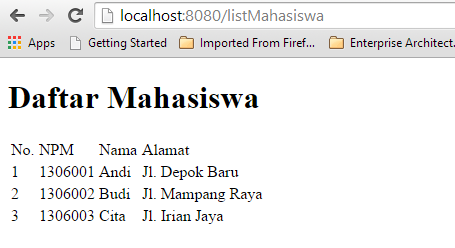
\includegraphics[
        width=0.6\textwidth
    ]{img/hasil-list-mhs.png}
    \caption{Halaman daftar mahasiswa yang dibuat menggunakan ABS}
    \label{fig:htmlDaftarMhs}
\end{figure}

Sampai pada tahap ini, penulis telah berhasil memetakan modul-modul ABS yang dibuat kedalam komponen MVC untuk menghasilkan sebuah halaman web. Namun penulis masih menemukan banyak kekurangan dalam pembuatan komponen MVC ini yang salah satu diantaranya adalah ketika kita membuat komponen view (modul \texttt{MahasiswaListView}). Jika melihat kode \ref{lst:absModuleMhsView} di atas, kode HTML yang dibuat oleh penulis masih berupa \texttt{String} yang disambung-sambung. Hal ini tentunya sangat tidak efektif terlebih lagi jika penulis ingin membuat sebuah halaman web yang lebih kompleks. Oleh karena itu, dibutuhkan adanya solusi lain untuk dapat membuat komponen view ini menjadi lebih mudah dibuat dan dikelola.

\section{Memperbaiki komponen view menggunakan HTML Template Engine}

Berdasarkan hasil evaluasi pada percobaan sebelumnya, penulis merasa perlu untuk mengganti metode yang penulis lakukan dalam membuat komponen view dengan menggunakan ABS. Setelah dikaji lebih jauh lagi, penulis menyadari bahwa standar yang berlaku dalam membuat sebuah halaman web adalah dengan menggunakan HTML. Pada saat penulis membuat komponen view dengan menggunakan ABS untuk menghasilkan HTML, proses pembuatan komponen view menjadi lebih rumit dan kurang fleksibel. Oleh karena itu, penulis membuat keputusan untuk meninggalkan ABS dan beralih ke kode HTML murni ketika membuat komponen view aplikasi.\\

Salah satu pendekatan yang dapat dilakukan utuk mengintegrasikan ABS dengan HTML adalah dengan menggunakan HTML \textit{template engine}. Secara singkat HTML \textit{template engine} adalah sebuah perangkat lunak yang dapat digunakan para pengembang perangkat lunak untuk dapat menyematkan objek ke dalam sebuah HTML dengan menggunakan sintaks tambahan. Dengan menggunakan perangkat lunak ini, penulis dapat langsung menyematkan modul \texttt{Mahasiswa} yang telah penulis buat kedalam sebuah halaman HTML. Dalam penelitian ini, penulis menggunakan HTML \textit{template engine} berbasis JAVA yaitu Thymeleaf (http://thymeleaf.org).

\begin{figure}
    \centering
    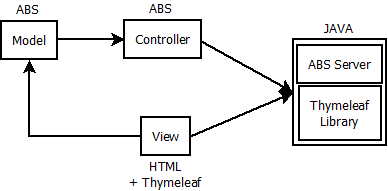
\includegraphics[
        width=0.8\textwidth]{img/alur-thymeleaf.png}
    \caption{Integrasi ABS, JAVA dan Thymeleaf}
    \label{fig:integrasiThymeleaf}
\end{figure}

Seperti yang terlihat pada gambar \ref{fig:integrasiThymeleaf}, dalam kasus ini penulis tidak langsung memanggil komponen View melalui Controller seperti yang penulis lakukan pada kode \ref{lst:absModuleMhsController}. Hal ini dilakukan karena komponen View yang dibuat dengan menggunakan thymeleaf murni menggunakan sintaks HTML sehingga tidak dapat dibuat objeknya. Penggunaan HTML dalam membuat komponen View tentunya akan mempermudah para pengembang perangkat lunak dalam membuat komponen View serta memubuat komponen view menjadi lebih rapih dan mudah dibaca. berikut perubahan pada komponen view yang penulis buat dengan menggunakan thymeleaf:

\begin{lstlisting}[
caption=Komponen View menggunakan HTML dan Thymeleaf,
label={lst:viewMhsListHTML},
escapeinside={@}{@}
]
<!DOCTYPE html>
<html>
<body>
	<h1>Daftar Mahasiswa</h1>
	<table>
		<thead>
			<tr>
				<td>No.</td>
				<td>NPM</td>
				<td>Nama</td>
				<td>Alamat</td>
			</tr>
		</thead>
		<tbody>
			<tr th:each="mahasiswa: ${mahasiswaList}">
				<td><p th:text="${#ids.seq('')}"></p></td>
				<td><p th:text="${mahasiswa.npm}"></p></td>
				<td><p th:text="${mahasiswa.nama}"></p></td>
				<td><p th:text="${mahasiswa.alamat}"></p></td>
			</tr>
		</tbody>
	</table>
</body>
</html>
\end{lstlisting}

Seperti yang terlihat pada kode \ref{lst:viewMhsListHTML} di atas, penulis membuat sebuah halaman web yang equivalent dengan kode \ref{lst:absModuleMhsView} hanya saja kode ini dibuat dengan menggunakan sintaks HTML dan thymeleaf. Jika kita lihat kode \ref{lst:viewMhsListHTML} baris \ref{lst:thymeStartLoop} - \ref{lst:thymeEndLoop} terdapat sebuah sintaks yang bukan standar HTML, sintaks tersebut merupakan sintaks dari thymeleaf (bisanya dintadi dengan \texttt{th:}). Tujuan dari penggunaan sintaks tersebut adalah untuk melakukan iterasi pada sebuah \texttt{List} untuk kemudian menampilkan seluruh atribut dari objek yang berada di dalam \texttt{List} tersebut.\\

Sampai pada tahap ini penulis telah berhasil memperbaiki komponen view dari yang sebelumnya menggunakan ABS menjadi HTML dan thymeleaf sehingga membuat komponen ini menjadi lebih mudah untuk didefinisikan dan lebih sesuai dengan kebiasaan para pengembang. Akan tetapi perubahan ini belum dapat diintegrasikan secara langsung dengan komponen-komponen lainnya karena masih banyak penyesuaian yang harus dilakukan baik di tingkat \textit{web server} maupun di komponen MVC lainnya. Oleh karena itu, langkah selanjutnya yang dilakukan oleh penulis adalah mengubah \textit{web server} dan komponen MVC lainnya agar sesuai dengan implementasi komponen View yang terbaru.

\section{Mengintegrasikan Thymeleaf dengan Web Server dan ABS}

Walaupum ABS dapat dikompilasi kedalam bentuk JAVA dan Thymeleaf juga merupakan komponen perangkat lunak yang berbasis JAVA, penulis tidak dapat mengintegrasikan dua hal tersebut secara langsung di dalam Class JAVA hasi kompilasi ABS. Hal ini terjadi karena penulis tidak ingin melakukan modifikasi terhadap Class JAVA tersebut dikarenakan Class JAVA ini merupakan \textit{auto generated file} sehingga kodenya akan selalu berubah. Oleh karena itu, penulis memutuskan untuk mengintegrasikan Thymeleaf dengan komponen MVC ABS di tingkat \textit{web server}. berikut adalah langkah-langkah yang penulis ambil dalam proses integrasinya:

\begin{enumerate}
    \item Pada saat \textit{web server} menerima \textit{request} dari \textit{web browser}, \textit{web server} akan memanggil komponen Controller ABS (yang sudah dikompilasi menjadi JAVA) yang diinginkan.
    \item Komponen Controller tersebut nantinya akan memberikan data (komponen Model) dan lokasi berkas HTML yang menjadi komponen View-nya.
    \item Setelah \textit{web server} menerima data dan lokasi berkas HTML dari komponen Controller, selanjutnya \textit{web server} akan mencari berkas HTML tersebut dan membuat sebuah \texttt{Context} untuk kemudian digabungkan dengan data yang diberikan.
    \item Setelah proses penggabungan selesai dan halaman web yang diinginkan sudah terbentuk, selanjutnya \textit{web server} akan memberikan halaman web tersebut kepada web browser.
\end{enumerate}

Berikut adalah modul \texttt{MMahasiswaController} yang sudah diubah sesuai dengan rencana implementasi di atas:

\begin{lstlisting}[
caption=Module \texttt{MMahasiswaController} yang disesuaikan untuk integrasi thymeleaf,
label={lst:absMhsControllerNew},
escapeinside={@}{@}
]
module Controller.MMahasiswaController;
import Mahasiswa, MahasiswaImpl from Model.MMahasiswa;

interface MahasiswaController
{
	Pair<String, List<Mahasiswa>> showMahasiswaList(); @\label{lst:absReturnType}@
}

class MahasiswaControllerImpl implements MahasiswaController
{
	Pair<String, List<Mahasiswa>> showMahasiswaList() @\label{lst:absReturnType2}@
	{
		...
		
		return Pair("list_mahasiswa", listMhs); @\label{lst:absReturnViewAndModel}@
	}
}
\end{lstlisting}

Terlihat pada kode \ref{lst:absMhsControllerNew} baris \ref{lst:absReturnViewAndModel}, penulis tidak lagi membuat \textit{instance} dari \texttt{MahasiswaListView} melainkan hanya mengembalikan lokasi berkas HTML yang menjadi komponen View-nya berserta dengan data Mahasiswa yang akan ditampilkan kedalam halaman web. Selain itu, pada bari \ref{lst:absReturnType} dan \ref{lst:absReturnType2} juga terdapat perubahan kode yaitu dari yang sebelumya \textit{method} \texttt{showMahasiswaList} hanya mengembalikan nilai \texttt{String} berubah menjadi \texttt{Pair(String, List<Mahasiswa>)}.

Setelah melakukan perubahan pada komponen Controller, berikutnya adalah melakukan perubahan pada \textit{web server}. Berikut adalah perubahan-perubahan pada web server yang penulis lakukan untuk mengintegrasikan thymeleaf dengan ABS:

\begin{lstlisting}[
caption=Perubahan pada kode \textit{web server},
label={lst:javaNewWebServer}
]
...

else if(protocols[1].equals("/listMahasiswa")) {
   	MahasiswaController_i controller = MahasiswaControllerImpl_c.__ABS_createNewObject(this);
   	Pair<ABSString, ABS.StdLib.List<Mahasiswa_i>> pair = controller.showMahasiswaList();
   	String view = pair.getArg(0).toString().replaceAll("\"", "");
   	
   	ABS.StdLib.List<Mahasiswa_i> absData = (ABS.StdLib.List<Mahasiswa_i>) pair.getArg(1);
   	ArrayList<Object> data = new ArrayList<Object>();
           		
	do
	{
		ABSObject head = (ABSObject) ABS.StdLib.head_f.apply(absData);
		data.add(head);
		
		absData = ABS.StdLib.tail_f.apply(absData);
	}
	while(!(absData instanceof ABS.StdLib.List_Nil));
	
	TemplateResolver templateResolver = new TemplateResolver();
    templateResolver.setTemplateMode("XHTML");
    templateResolver.setSuffix(".html");
    templateResolver.setResourceResolver(new ResourceResolver());
                
    TemplateEngine templateEngine = new TemplateEngine();
    templateEngine.setTemplateResolver(templateResolver);
                
	Context ctx = new Context();
	StringWriter writer = new StringWriter();
	ctx.setVariable("mahasiswaList", data);
	templateEngine.process(view, ctx, writer);
	
	out.println(writer);
}

...
\end{lstlisting}

\begin{lstlisting}[
caption=Class \texttt{ResourceResolver} sebagai tambahan pada \textit{web server},
label={lst:javaResourceResolver}
]
public class ResourceResolver implements IResourceResolver
{
	private static final String NAME = "ABSResourceResolver";
	
	@Override
	public String getName() 
	{
		// TODO Auto-generated method stub
		return NAME;
	}

	@Override
	public InputStream getResourceAsStream(TemplateProcessingParameters templateProcessingParameter,
			String resourceName) 
	{
		
		Validate.notNull(resourceName, "Resource name cannot be null");
		return ResourceResolver.class.getResourceAsStream("/" + resourceName);
	}

}
\end{lstlisting}

\section{Membuat Ant Script untuk mempermudah proses Compile dan Deployment}
Bagian ini menjelaskan tentang proses pembuatan ant script untuk mempermudah proses compile dan deployment dari yang sebelumnya menggunakan menu di eclipse menjadi ke terminal console.

\section{Menerima input POST dan GET dari web browser}
Bagian ini menjelaskan tentang eksperimen yang dilakukan oleh penulis dalam mencari tahu metode seperti apa yang dapat digunakan dalam menerima input HTTP POST dan GET dari web browser.

\section{Membuat Routing configuration}
Bagian ini menjelaskan tentang proses pembuatan routing configuration untuk memetakan setiap url kedalam class controller dan methodnya.
\chapter{Proses Penyusunan ABS MVC Framework}

Setelah melakukan berbagai eksperimen untuk memetakan ABS kedalam komponen-komponen MVC dan mengintegrasikannya dengan \textit{web server} sederhana, selanjutnya adalah menyusun hasil eksperimen-eksperimen tersebut agar menjadi satu kesatuan framework MVC ABS yang utuh. Ada beberapa poin yang akan disusun terkait pembuatan framework MVC ABS yang diantaranya adalah:

\begin{enumerate}
    \item Pengaturan struktur direktori.
    \item Menambahkan Ant Script untuk mempermudah proses kompilasi dan \textit{deployment}.
    \item Penambahan mekanisme konfigurasi URL \textit{routing}.
    \item Penambahan mekanisme untuk menangani HTTP POST dan GET data.
\end{enumerate}

\section{Pengaturan struktur direktori}

Struktur direkretori dalam sebuah framework MVC berperan dalam membantu para pengguna framework untuk mengatur peletakan setiap kode program yang mereka hasilkan sesuai dengan kategori / jenis dari kode program tersebut. Dengan adanya struktur direktori yang baik, akan membantu para pengembang perangkat lunak untuk dapat konsisten dalam meletakkan setiap kode program yang mereka hasilkan. berikut ini adalah struktur direktori dari framework MVC ABS:

\begin{itemize}
    \item \textbf{dist}: folder ini digunakan untuk menyimpan \textit{binary} dari aplikasi web yang sudah di compile.
    \item \textbf{src}: folder ini digunakan untuk menyimpan file ABS yang dibuat oleh para pengembang perangkat lunak. folder ini memiliki sub direktori "model", "view" dan "controller" yang digunakan untuk meletakkan komponen MVC yang dibuat. Selain itu, di dalam direktori ini juga terdapat sebuah direktori bernama "framework" yang berisi berkas kode program ABS yang digunakan untuk keperluan internal framework dan direktori "delta" yang digunakan untuk meletakan kode delta dalam proses penerapan \textit{delta modeling}.
    \item \textbf{lib}: folder ini berisi library yang dibutuhkan oleh framework MVC ABS untuk dapat meng-compile kode ABS dan mengubahnya ke dalam kode JAVA.
    \item \textbf{target}: folder ini digunakan sebagai tempat penampungan sementara ketika framework sedang melakukan proses kompilasi kode ABS.
\end{itemize}

\begin{figure}
    \centering
    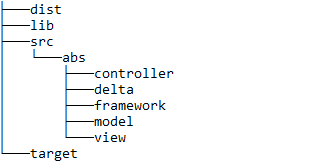
\includegraphics[width=0.4\textwidth]
        {img/struktur-direktori.png}
    \caption{Struktur Direktori ABS MVC Framework}
    \label{fig:strukturDirektori}
\end{figure}

Berdasarkan susunan direktori seperti yang terlihat pada Gambar \ref{fig:strukturDirektori} di atas, seluruh komponen MVC yang dibuat (misal: modul MMahasiswa, MMahasiswaController dan berkas HTML) akan diletakkan di dalam direktori \texttt{src/abs/(model, view, controller)}. Setelah seluruh komponen MVC diletakkan di dalam direktorinya masing-masing, nantinya framework MVC ini akan meng\textit{compile} seluruh kode ABS yang ada serta membungkusnya kedalam berkas JAVA \textit{archive} (jar) dan meletakannya di dalam direktori \texttt{dist}.\\

Sampai sejauh ini penulis telah berhasil melakukan penyusunan direktori untuk \textit{framework} MVC ABS. Hal berikutnya yang penulis lakukan adalah membuat sebuah \textit{script} yang akan digunakan untuk melakukan proses kompilasi dan \textit{deployment} secara otomatis.

\section{Pembuatan Ant Script Untuk Proses Kompilasi dan \textit{Deployment}}

Untuk mempermudah pengembang perangkat lunak dalam melakukan proses kompilasi dan \textit{deployment}, penulis membuat sebuah \textit{build script} dengan menggunakan Apache Ant \footnote{http://ant.apache.org/}. Tujuan dari dibuatnya \textit{build script} ini adalah agar para pengembang dapat menjalankan keseluruhan proses tersebut dengan hanya mengetikkan satu buah perintah pada \textit{terminal console}. Sebagian besar \textit{script} yang digunakan untuk proses kompilasi dan \textit{deployment} ini diadaptasi dari Ant Script yang telah dibuat oleh tim HATS \footnote{http://tools.hats-project.eu/core/anttasks.html}. berikut adalah \textit{build script} yang penulis buat untuk framework MVC ABS:

\begin{lstlisting}[
caption=Build script untuk framework MVC ABS berbasis Apache Ant,
label={lst:antBuildScript},
escapeinside={@}{@}
]
<?xml version="1.0" encoding="UTF-8"?>
<project name="ABS MVC" default="abs.compile.java" basedir="."
	xmlns:artifact="antlib:org.apache.maven.artifact.ant">

	<property name="lib" location="lib" />
	<property name="src" location="src" />
	<property name="target" location="target" />
	<property name="dist" location="dist" />

	<property name="src.abs" location="${src}/abs" />
	
	<property name="target.java.src" location="${target}/java/src" />
	<property name="target.java.bin" location="${target}/java/bin" />

	<property name="lib.abs" location="${lib}/absfrontend.jar" />
	
	<property name="server" location="../ABSServer" />
	<property name="server.web" location="${server}/web" />

	<path id="build.abs.classpath">
		<pathelement location="${lib.abs}" />
	</path>

	<fileset dir="${src.abs}" id="src.abs.files">
		<include name="**/*.abs" />
	</fileset>
	
	<pathconvert property="src.abs.fileargs" refid="src.abs.files"
		pathsep=" " />
	
	<target name="clean" description="Removes all generated files"> @\label{lst:targetClean}@
		<delete failonerror="false" includeemptydirs="true">
			<fileset dir="${target}" />
		</delete>
	</target>

	<target name="prepare" depends="clean"> @\label{lst:targetPrepare}@
		<mkdir dir="${target.java.src}" />
		<mkdir dir="${target.java.bin}" />
	</target>

	<target name="abs.typecheck" depends="prepare"> @\label{lst:targetTypeCheck}@
		<java classname="abs.frontend.parser.Main" fork="true"
			failonerror="true" classpathref="build.abs.classpath">
			<arg line="${src.abs.fileargs}" />
		</java>
	</target>

	<target name="abs.generate.java" description="Generates Java code" @\label{lst:targetABSGenerateJava}@
		depends="clean,prepare">
		<echo>FILE: ${src.abs.fileargs}</echo>
		<java classname="abs.backend.java.JavaBackend" fork="true"
			failonerror="true" classpathref="build.abs.classpath">
			<arg line="${src.abs.fileargs}" />
			<arg value="-sourceonly" />
			<arg value="-d" />
			<arg value="${target.java.src}" />
		</java>
	</target>

	<target name="abs.compile.java" depends="abs.generate.java"> @\label{lst:targetABSCompileJava}@
		<javac classpathref="build.abs.classpath" srcdir="${target.java.src}"
			destdir="${target.java.bin}" />
			
		<copy todir="${target.java.bin}/View">
			<fileset dir="${src.abs}/view" />
		</copy>
	</target>
	
	<target name="abs.build.jar" depends="abs.compile.java"> @\label{lst:targetABSBuildJar}@
		<jar 
			destfile="${dist}/app.jar"
			basedir="${target.java.bin}" />
	</target>
	<target name="abs.deploy" depends="abs.build.jar"> @\label{lst:targetABSDeploy}@
		<copy todir="${server.lib}">
			<file file="${dist}/app.jar" />
		</copy>
	</target>
</project>
\end{lstlisting}

Pada dasarnya \textit{build script} yang penulis buat merupakan kumpulan perintah-perintah yang mendefinisikan alur dari proses kompilasi sampai \textit{deployment} seperti yang terlihat pada Kode \ref{lst:antBuildScript} baris \ref{lst:targetClean}, \ref{lst:targetPrepare}, \ref{lst:targetTypeCheck}, \ref{lst:targetABSGenerateJava}, \ref{lst:targetABSCompileJava}, \ref{lst:targetABSBuildJar} dan \ref{lst:targetABSDeploy}. Berdasarkan kode-kode tersebut, terlihat bahwa ada 7 (tujuh) buah perintah yang masing-masing saling memiliki ketergantungan sehingga membentuk sebuah rangkaian alur seperti yang terlihat pada Gambar \ref{fig:buildScriptFlow}. Berikut adalah rangkaian alur yang penulis definisikan pada \textit{build script} tersebut:

\begin{enumerate}
    \item \textbf{clean:} Perintah ini digunakan untuk membersihkan seluruh berkas-berkas hasil \textit{auto-generated}.
    \item \textbf{prepare:} Perintah ini digunakan untuk membuat direktori-direktori tambahan yang dibutuhkan pada saat proses kompilasi.
    \item \textbf{abs.typecheck:} Perintah ini digunakan untuk memvalidasi kode ABS yang akan di\textit{compile}.
    \item \textbf{abs.generate.java:} Perintah ini digunakan untuk menghasilkan kode JAVA dari kode ABS yang dibuat.
    \item \textbf{abs.compile.java:} Perintah ini digunakan untuk meng\textit{compile} seluruh kode JAVA hasi kompilasi dari kode ABS yang dibuat.
    \item \textbf{abs.build.jar:} Perintah ini digunakan untuk membungkus seluruh berkas hasil kompilasi ke dalam sebuah berkas JAVA Archive.
    \item \textbf{abs.deploy:} Perintah ini digunakan untuk meletakan berkas .jar yang telah dihasilkan kedalam \textit{web server}.
\end{enumerate}

\begin{figure}
    \centering
    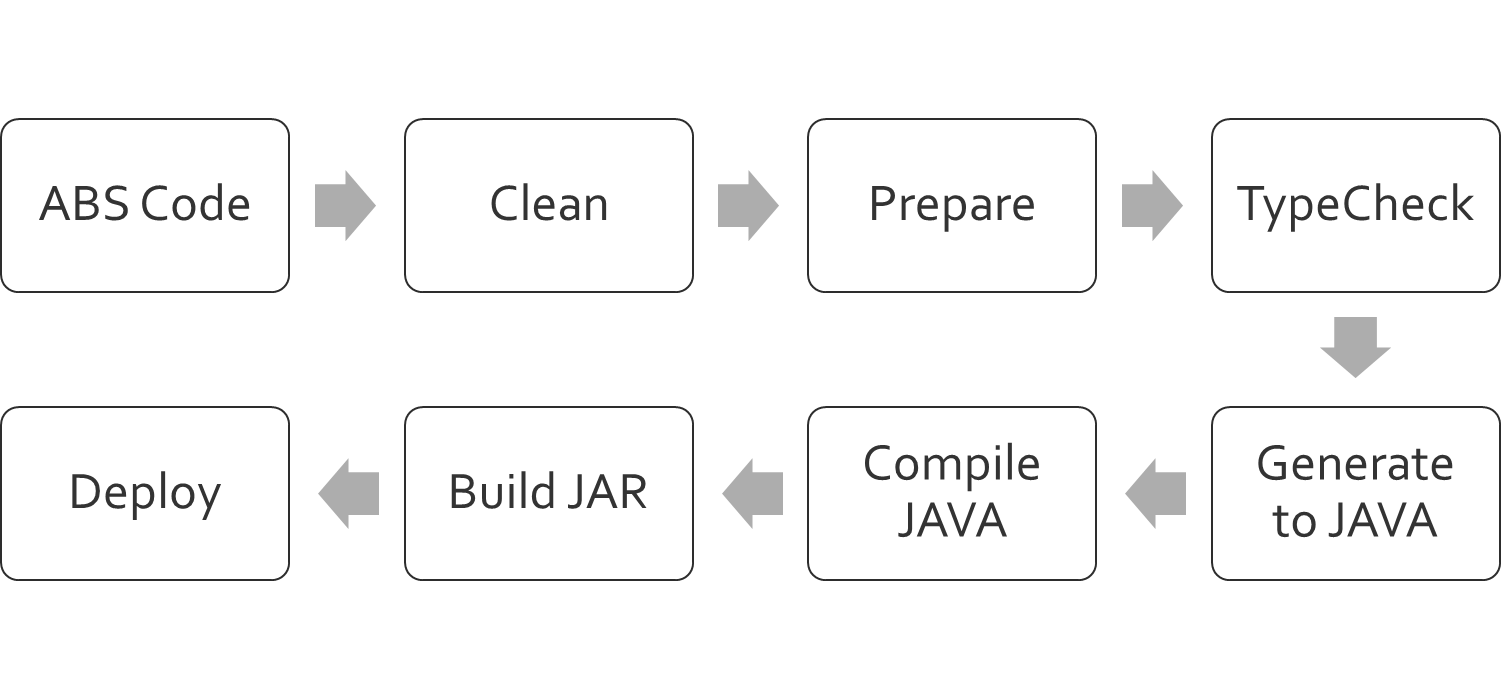
\includegraphics[width=0.8\textwidth]{img/build-script-flow.png}
    \caption{Alur dalam proses kompilasi dan \textit{deployment}}
    \label{fig:buildScriptFlow}
\end{figure}

Dengan menggunakan \textit{build script} yang sudah dibuat, para pengguna \textit{framework} hanya perlu mengetikkan perintah \texttt{ant -Dabsproduct=Default abs.deploy} dari dalam direktori framework untuk menjalankan keseluruhan proses kompilasi dan \textit{deployment} ABS MVC Framework.

Sampai pada tahap ini penulis telah berhasil menyusun direktori dan membuat \textit{build script} dengan menggunakan Apache Ant untuk mempermudah proses kompilasi dan \textit{deployment} pada \textit{framework} MVC ABS. langkah selanjutnya adalah menambahkan mekanisme konfigurasi URL \textit{routing} dan mengatasi HTTP POST dan GET data untuk lebih menyempurnakan lagi \textit{framework} MVC ABS yang dibuat.

\section{Penambahan Mekanisme Konfigurasi Pemetaan URL}

Jika kita melihat kembali Kode \ref{lst:javaNewWebServer} \textit{web server} di atas, dapat terlihat bahwa penulis masih menggunakan \texttt{if - else - elseif} dalam melakukan pemetaan antara URL dengan komponen Controller yang akan dipanggil. Tentunya hal ini sangat tidak efektif karena ketika terjadi penambahan komponen Controller, tentunya penulis harus menambahkan kembali blok \texttt{elsif} di dalam kode \textit{web server} untuk menambahkan pemetaan baru terhadap komponen Controller tersebut. Untuk membuat \textit{framework} ABS MVC lebih fleksibel terhadap perubahan, maka penulis membuat sebuah mekanisme di dalam \textit{framework} agar pengguna \textit{framework} MVC ABS dapat mendefinisikan pemetaannya sendiri langsung dari \textit{framework}.\\

Pendekatan yang penulis lakukan untuk dapat menyediakan fitur konfigurasi pemetaan URL tersebut adalah dengan membuat sebuah modul ABS khusus yang bernama \texttt{RouteConfig}. Modul ini berisikan daftar URL beserta nama komponen Controller dan \textit{method} yang akan dicocokan dengan menggunakan mekanisme \textit{pattern matching}. Modul ini nantinya akan dipanggil secara otomatis oleh \textit{web server} pada saat menerima \textit{request} dari \textit{web browser}. Tujuan dari pemanggilan modul ini oleh \textit{web server} adalah untuk mengetahui komponen Controller dan \textit{method} mana yang harus dipanggil oleh \textit{web server} untuk dapat menghasilkan halaman web yang diinginkan. Berikut adalah modul \texttt{RouteConfig} yang penulis sediakan untuk membantu para pengguna \textit{framework} dalam memetakan URL dengan Controller yang dibuat.

\begin{minipage}{\linewidth}
\begin{lstlisting}[
caption=Modul \texttt{RouteConfig} untuk pemetaan URL,
label={lst:absRouteConfig},
escapeinside={!}{!}
]
module ABS.Framework.Route;

interface RouteConfig
{
	String route(String url);
}

class RouteConfigImpl implements RouteConfig
{
	String route(String url)
	{
		String result = case url !\label{lst:startPatternMatching}!
		{
			"/product/index.abs" => "Controller.Product.ProductControllerImpl@index";
			"/product/add.abs" => "Controller.Product.ProductControllerImpl@addProduct"; !\label{lst:contohRouteConfig}!
			"/product/details.abs" => "Controller.Product.ProductControllerImpl@productDetails";
			"/product/list.abs" => "Controller.Product.ProductControllerImpl@productList";
			_ => ""; //default pattern
		}; !\label{lst:endPatternMatching}!
		
		return result;
	}
}
\end{lstlisting}
\end{minipage}

Seperti yang terlihat pada Kode \ref{lst:absRouteConfig} baris \ref{lst:startPatternMatching} sampai \ref{lst:endPatternMatching} di atas, penulis mendefinisikan 4 (empat) buah pemetaan URL dengan komponen Controller dan \textit{method}nya. Konvensi yang digunakan dalam mendefinisikan pemetaan URL tersebut adalah \texttt{[nama modul].[nama class]@[nama method]}. Sebagai contoh, pada Kode \ref{lst:absRouteConfig} baris \ref{lst:contohRouteConfig} di atas terlihat penulis memetakan sebuah URL \texttt{/product/add.abs} dengan sebuah komponen Controller bernama \texttt{ProductControllerImpl} yang berada di dalam modul \texttt{Controller.Product} dan memanggil \textit{method} \texttt{addProduct}. Dengan menggunakan mekanisme seperti ini, pengguna framework dapat langsung memetakan URL dengan komponen Controller yang dibuat tanpa harus mengubah kode sumber dari \textit{web server}.\\

Berikut ini adalah diagram alur pemanggilan modul \texttt{RouteConfig} oleh \textit{web server} dalam menghasilkan sebuah halaman web beserta penjelasannya.

\begin{figure}
    \centering
    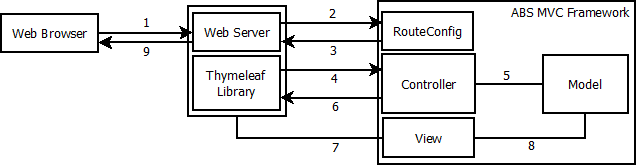
\includegraphics[width=0.8\textwidth]{img/absmvc_flow.png}
    \caption{Diagram alur pemanggilan Controller melalui \texttt{RouteConfig}}
    \label{fig:diagramABSMVCRouteConfig}
\end{figure}

Penjelasan:
\begin{enumerate}
    \item \textit{Web browser} mengirimkan HTTP \textit{request} kepada \textit{web browser} seperti misalnya \texttt{GET /product/add.abs HTTP/1.1}.
    \item \textit{Web server} akan mengambil segmen yang berisi \textit{path} \texttt{/product/add.abs} kepada modul \texttt{RouteConfig}.
    \item Modul \textit{RouteConfig} akan mencocokan \textit{path} yang diberikan dengan menggunakan \textit{pattern matching} untuk kemudian memberikan hasilnya berupa nama Controller dan \textit{method} yang harus dipanggil (misal: \texttt{Controller.Product.ProductControllerImpl@addProduct})kepada \textit{web server}.
    \item \textit{Web server} memanggil controller dan \textit{method} sesuai yang diberikan oleh modul \texttt{RouteConfig}.
    \item Controller menyiapkan data-data yang akan ditampilkan di halaman web.
    \item Controller memberikan data (Model) dan nama berkas HTML (View) untuk kemudian diproses oleh \textit{web server}.
    \item \textit{Web server} akan mencari dan memproses berkas HTML sesuai dengan nama yang diberikan oleh Controller.
    \item \textit{Web server} mengintegrasikan berkas HTML tersebut dengan data yang diberikan untuk menghasilkan sebuah halaman web.
    \item \textit{Web server} memberikan halaman web yang telah berhasil dibuat kepada \textit{web browser}.
\end{enumerate}

Sampai pada tahap ini penulis telah berhasil membuat modul ABS yang dapat digunakan untuk mengkonfigurasi pemetaan URL yang diberikan oleh \textit{web server} dengan komponen Controller yang dibuat. Dengan menggunakan cara ini, pengguna \textit{framework} tidak perlu mengubah kode sumber dari \textit{web browser} untuk melakukan proses pemetaan tersebut. Hal yang akan dilakukan selanjutnya oleh penulis adalah menambahkan mekanisme untuk menangani HTTP POST dan GET \textit{input} dari \textit{web browser}.

\section{Penambahan Mekanisme Penanganan HTTP POST dan GET Data}

Menangani HTTP POST dan GET data merupakan salah satu fitur yang sangat penting dalam membangun sebuah aplikasi berbasis web. Melalui mekanisme ini, para pengguna dapat berinteraksi dengan aplikasi web yang dibuat sehingga membuat konten aplikasi tersebut menjadi lebih dinamis. Untuk dapat menghasilkan sebuah \textit{framework} MVC yang utuh, tentunya fitur ini harus disediakan untuk mempermudah pengembang aplikasi web dalam menerima dan memproses data yang diberikan oleh para pengguna. Pendekatan yang dapat dilakukan untuk dapat mengimplementasikan fitur ini kedalam \textit{framework} MVC ABS adalah dengan cara memberikan HTTP POST dan GET data tersebut secara langsung dari \textit{web server} kepada \textit{framework} dalam bentuk objek.

Berikut ini adalah langkah-langkah yang penulis lakukan dalam memberikan HTTP POST dan GET data yang diterima dari \textit{web browser} kepada \textit{framework} MVC ABS:

\begin{enumerate}
    \item \textit{Web browser} memberikan data kepada \textit{web server} dengan menggunakan protokol HTTP GET atau POST (seperti yang terlihat pada Kode \ref{lst:httpGETInput} dan \ref{lst:httpPOSTInput}).
    \item \textit{Web server} mengurai protokol HTTP tersebut untuk mendapatkan data-data yang diberikan dan membungkusnya kedalam sebuah objek.
    \item \textit{Web server} memberikan objek yang berisi data-data tersebut kepada \textit{framework} MVC ABS bersamaan dengan pemanggilan komponen Controller.
    \item Komponen Controller menerima data yang diberikan dan memproses POST atau GET data tersebut untuk menghasilkan data model yang dibutuhkan.
\end{enumerate}

\begin{lstlisting}[
language=TeX,
caption=Contoh HTTP GET \textit{header} beserta datanya,
label={lst:httpGETInput},
escapeinside={@}{@}
]
GET /product/details.abs?product_sku=00188&product_name=FMSE+Dining+Set&description=Beautiful+and+Cute+Dining+Set&price=250000 HTTP/1.1 @\label{lst:httpGETData}@
Host: localhost:8080
Connection: keep-alive
Accept: text/html,application/xhtml+xml,application/xml;q=0.9,image/webp,*/*;q=0.8
User-Agent: Mozilla/5.0 (Windows NT 6.3; WOW64) AppleWebKit/537.36 (KHTML, like Gecko) Chrome/39.0.2171.71 Safari/537.36
Referer: http://localhost:8080/product/add.abs
Accept-Encoding: gzip, deflate, sdch
Accept-Language: en-US,en;q=0.8,id;q=0.6
\end{lstlisting}

\begin{lstlisting}[
language=TeX,
caption=Contoh HTTP POST \textit{header} beserta datanya,
label={lst:httpPOSTInput},
escapeinside={@}{@}
]
POST /product/details.abs HTTP/1.1
Host: localhost:8080
Connection: keep-alive
Content-Length: 101 @\label{lst:contentLength}@
Cache-Control: max-age=0
Accept: text/html,application/xhtml+xml,application/xml;q=0.9,image/webp,*/*;q=0.8
Origin: http://localhost:8080
User-Agent: Mozilla/5.0 (Windows NT 6.3; WOW64) AppleWebKit/537.36 (KHTML, like Gecko) Chrome/39.0.2171.71 Safari/537.36
Content-Type: application/x-www-form-urlencoded
Referer: http://localhost:8080/product/add.abs
Accept-Encoding: gzip, deflate
Accept-Language: en-US,en;q=0.8,id;q=0.6

product_sku=00188&product_name=FMSE+Dining+Set&description=Beautiful+and+Cute+Dining+Set&price=250000 @\label{lst:httpPOSTData}@
\end{lstlisting}

Seperti yang terlihat pada Kode \ref{lst:httpGETInput} dan \ref{lst:httpPOSTInput} di atas, terdapat sedikit perbedaan pada protokol HTTP GET dan POST dalam memberikan data. Pada protokol HTTP GET data langsung diberikan pada URL seperti yang terlihat pada Kode \ref{lst:httpGETInput} baris \ref{lst:httpGETData} sedangkan protokol HTTP POST data diberikan secara terpisah dari bagian HTTP \textit{header} dengan memberikan tambahan informasi \texttt{Content-Length} untuk mengetahui panjang data yang diberikan dalam bentuk \texttt{byte} (lihat Kode \ref{lst:httpPOSTInput} baris \ref{lst:contentLength} dan \ref{lst:httpPOSTData}). Dikarenakan letak data pada kedua protokol tersebut berbeda, dibutuhkan adanya dua buah implementasi kode pada \textit{web server} seperti yang ditunjukan pada Kode \ref{lst:javaParseHTTPData} di bawah ini:

\begin{lstlisting}[
firstnumber=81,
caption=Implementasi penguraian protokol POST dan GET pada \textit{web server},
label={lst:javaParseHTTPData},
escapeinside={@}{@}
]
...

if(requestMethod.equals("POST"))
{
   	HashMap<String, String> requestHeaders = request.getHeaders();
   	Integer contentLength = Integer.parseInt(requestHeaders.get("Content-Length"));
   	char[] buffer = new char[contentLength];
   	in.read(buffer);
   	
   	String inputString = URLDecoder.decode(new String(buffer), "UTF-8");
   	String[] inputs = inputString.split("&");
   	
   	HashMap<String, String> requestInputs = new HashMap<String, String>();
   	for (String input : inputs) 
   	{
		String key = input.split("=")[0];
		String value = input.split("=")[1];
		requestInputs.put(key, value);
	}
            	
    request.setRequestInputs(requestInputs);
}
else if(requestMethod.equals("GET"))
{
   	String uri = request.getRequestUri();
   	String[] splittedUri = uri.split("\\?");
   	
   	if(splittedUri.length > 1)
   	{
   		String requestSegment = splittedUri[0];
   		String inputSegment = splittedUri[1];
   		
   		request.setRequestUri(requestSegment);
   		String[] inputData = inputSegment.split("&");

   		HashMap<String, String> requestInputs = new HashMap<String, String>();
   		for (String input : inputData) 
   		{
   			String key = URLDecoder.decode(input.split("=")[0], "UTF-8");
   			String value = URLDecoder.decode(input.split("=")[1], "UTF-8");
   			
   			requestInputs.put(key, value);
		}
            		
   		request.setRequestInputs(requestInputs);
   	}
}

...
\end{lstlisting}

Seperti yang terlihat pada Kode \ref{lst:javaParseHTTPData} baris diatas, pada saat penulis menguraikan data pada protokol HTTP POST dan GET, penulis mengumpulkan data-data tersebut kedalam sebuah \texttt{HashMap<String, String>}. Tujuan dari pembuatan \texttt{HashMap} tersebut adalah untuk mengumpulkan seluruh data yang dikirimkan oleh \textit{web browser} untuk kemudian diberikan kepada \textit{framework} MVC ABS. Mekanisme yang digunakan dalam mengirimkan HTTP POST dan GET data tersebut adalah dengan membuat sebuah modul baru pada \textit{framework} MVC ABS yang bernama \texttt{HTTPRequest}. Berikut adalah modul ABS \texttt{HTTPRequest} telah penulis buat dalam mengimplementasikan hal tersebut.

\begin{lstlisting}[
caption=Modul \texttt{ABSHttpRequest},
label={lst:absHttpRequest}
]
interface ABSHttpRequest
{
	String getInput(String key);
}

class ABSHttpRequestImpl(Map<String, String> requestInput) implements ABSHttpRequest
{
	String getInput(String key)
	{
		String value = fromJust(lookup(requestInput, key));
		return value;
	}
}
\end{lstlisting}

Dengan adanya tambahan modul \texttt{ABSHttpRequest}, para pengguna \textit{framework} MVC ABS dapat dengan mudah untuk menerima dan memproses setiap \textit{input} yang diberikan oleh pengguna aplikasi. Untuk dapat memproses \textit{input} yang diberikan, diperlukan adanya sedikit perubahan terkait cara mendefinisikan sebuah \textit{method} pada komponen Controller yang dibuat. Perubahan yang harus dilakukan adalah menyertakan modul \texttt{ABSHttpRequest} tersebut sebagai parameter dalam setiap \textit{method} yang dibuat. Berikut adalah contoh \textit{method} pada komponen Controller yang sudah mengimplementasikan modul \texttt{ABSHttpRequest}.

\begin{minipage}{\linewidth}
    \begin{lstlisting}[
    firstnumber=24,
    caption=Contoh \textit{method} yang sudah mengimplementasikan \texttt{ABSHttpRequest},
    label={lst:absGetHTTPInput},
    escapeinside={@}{@}
    ]
    ...
    
    Pair<String, List<Product>> productDetails(ABSHttpRequest request)
    {
    	String sku = request.getInput("product_sku"); @\label{lst:absGetInputParam}@
    	String name = request.getInput("product_name");
    	String description = request.getInput("description");
    	String price = request.getInput("price"); @\label{lst:absGetInputParam2}@
    	
    	Product myProduct = new local ProductImpl(sku, name, description, price);
    	List<Product> dataList = Nil;
    	dataList = appendright(dataList, myProduct);
    	
    	return Pair("product/details", dataList);
    }
    
    ...
    \end{lstlisting}
\end{minipage}

Seperti yang terlihat pada Kode \ref{lst:absGetHTTPInput} baris \ref{lst:absGetInputParam} sampai \ref{lst:absGetInputParam2}, penulis dapat mengambil \textit{input} data yang diberikan oleh pengguna dengan cara memanggil \textit{method} \texttt{getInput(namaParameter)} yang sudah disediakan oleh modul \texttt{ABSHttpRequest}. Adapun nama parameter yang menjadi kunci dalam mengambil \textit{input} data yang diinginkan adalah dari atribute \texttt{name} pada tag \texttt{<input>} yang disediakan oleh HTML (lihat Kode \ref{lst:viewWithForm} dan \ref{lst:absGetHTTPInput}). Berikut ini adalah contoh halaman HTML yang ditujukan untuk mengirimkan HTTP POST data untuk kemudian di proses oleh Controller pada Kode \ref{lst:absGetHTTPInput} diatas.

\begin{lstlisting}[
caption=Contoh halaman HTML yang mengandung \texttt{<form>},
label={lst:viewWithForm}
]
<form method="POST" action="/product/details.abs">
<table>
	<tbody>
		<tr>
			<td>Product SKU</td>
			<td>:</td>
			<td><input type="text" name="product_sku" /></td>
		</tr>
		<tr>
			<td>Product Name</td>
			<td>:</td>
			<td><input type="text" name="product_name" /></td>
		</tr>
		<tr>
			<td>Description</td>
			<td>:</td>
			<td><input type="text" name="description" /></td>
		</tr>
		<tr>
			<td>Price</td>
			<td>:</td>
			<td><input type="text" name="price" /></td>
		</tr>
	</tbody>
</table>
<input type="submit" value="Submit" />
</form>
\end{lstlisting}

Sampai pada tahap ini penulis telah berhasil menambahkan fitur untuk penanganan HTTP POST dan GET data yang diberikan oleh \textit{web browser}. Dengan demikian, \textit{framework} MVC ABS yang dibuat saat ini sudah berhasil menjadi sebuah \textit{famework} yang utuh dan dapat digunakan untuk membuat sebuah aplikasi berbasis web. 

\section{Hasil Akhir}

Setelah melakukan banyak perubahan pada \textit{framework} dan kode \textit{web server}, diperoleh dua buah hasil akhir dari proses eksperimen yang penulis lakukan. Adapun hasil akhir dari proses eksperimen ini adalah dua buah produk yang bernama ABS Server dan ABS MVC Framework. Berikut adalah detail kedua buah produk tersebut:

\subsection{ABS MVC Framework}

ABS MVC Framework merupakan sebuah \textit{framework} yang ditujukan untuk membantu para pengembang perangkat lunak dalam membangun sebuah aplikasi web berbasis ABS dengan pola Model-View-Controller (MVC). Konten dari \textit{framework} ini adalah berupa kumpulan direktori, dua buah modul ABS dan sebuah \textit{build script} yang dapat membantu para pengembang perangkat lunak dalam membangun aplikasi web yang diinginkan. Adapun detail konten dari ABS MVC Framework adalah sebagai berikut:

Direktori:
\begin{itemize}
    \item \texttt{src/abs/controller}: merupakan direktori yang digunakan untuk meletakan modul Controller ABS yang dibuat.
    \item \texttt{src/abs/view}: merupakan direktori yang digunakan untuk menyimpan halaman HTML yang dibuat.
    \item \texttt{src/abs/model}: merupakan direktori yang digunakan untuk meletakan setiap modul model yang dibuat.
    \item \texttt{src/abs/framewok}: merupakan direktori yang digunakan untuk meletakan modul internal \textit{framework} yang dibuat oleh penulis seperti modul \texttt{ABSHttpRequest} dan \texttt{RouteConfig}.
\end{itemize}

Modul ABS:
\begin{itemize}
    \item \texttt{ABSHttpRequest}: modul ini digunakan untuk mengambil HTTP POST dan GET data yang diterima oleh \textit{web server}.
    \item \texttt{RouteConfig}: modul ini digunakan untuk melakukan pemetaan URL dengan Controller dan \textit{method} yang dibuat.
\end{itemize}

Lain-lain:
\begin{itemize}
    \item \texttt{build.xml}: merupakan \textit{build script} yang dibuat dengan menggunakan Apache Ant dengan tujuan untuk memudahkan pengguna dalam proses kompilasi dan \textit{deployment}.
\end{itemize}

\begin{figure}
    \centering
    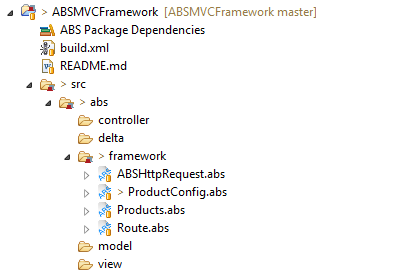
\includegraphics[width=0.6\textwidth]{img/abs-mvc-framework.png}
    \caption{Hasil akhir dari ABS MVC Framework}
    \label{fig:absMVCFramework}
\end{figure}

\subsection{ABS Server}

ABS Server merupakan sebuah \textit{web server} sederhana dibuat dengan tujuan untuk mencoba aplikasi web yang dibuat dengan menggunakan ABS MVC Framework. Fitur yang dimiliki oleh ABS Server ini antara lain adalah:

\begin{itemize}
    \item Menerima HTTP \textit{request} dari \textit{web browser} dan memprosesnya bersama dengan ABS MVC Framework untuk menghasilkan sebuah halaman web.
    \item Menerima HTTP POST dan GET data yang dikirim oleh \textit{web browser} dan meneruskannya ke ABS MVC Framework.
    \item Melakukan konversi tipe data \texttt{ABSString} kedalam JAVA String termasuk membersihkan tanda kutip "'" yang melekat pada setiap data bertipe \texttt{ABSString}.
    \item Melakukan konversi tipe data \texttt{ABS.StdLib.List} kedalam JAVA \texttt{ArrayList}.
\end{itemize}

Berikut ini adalah penjelasan dari masing-masing \textit{source code} yang ada di dalam ABS Server:

\begin{itemize}
    \item \texttt{HttpRequest.java}: Class JAVA ini merupakan Class pembantu yang digunakan untuk menyimpan seluruh informasi \textit{request} dari \textit{web browser} termasuk HTTP POST dan GET data untuk kemudian diberikan kepada ABS Framework.
    \item \texttt{HttpServer.java}: Class JAVA ini merupakan Class utama pada ABS Server. Melalui Class inilah aplikasi ABS Server berjalan.
    \item \texttt{RequestHandler.java}: Class JAVA ini berfungsi untuk memproses setiap \textit{request} yang diberikan oleh \textit{web browser} dan menyampaikannya kepada ABS MVC Framework untuk dapat menghasilkan sebuah halaman web.
    \item \texttt{ResourceResolver.java}: Class JAVA ini berfungsi untuk mengambil berkas HTML sesuai dengan lokasi berkas yang diberikan oleh modul \texttt{RouteConfig} dan mengubahnya menjadi JAVA \texttt{InputStream} untuk kemudian diproses oleh Thymeleaf.
    \item \texttt{DataTransformer.java}: Class JAVA ini berfungsi untuk melakukan konversi tipe data ABS kedalam tipe data JAVA. Untuk saat ini, tipe data yang sudah dikonversi adalah \texttt{ABSString} dan \texttt{ABS.StdLib.List}
\end{itemize}

\begin{figure}
    \centering
    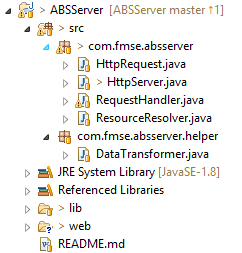
\includegraphics[width=0.6\textwidth]{img/abs-server-source.png}
    \caption{Hasil akhir dari ABS Server}
    \label{fig:absServer}
\end{figure}

Dalam penggunaanya, ABS Server ini telah penulis \textit{compile} dan diarsipkan kedalam berkas JAVA Archive (.jar) bernama \texttt{absserver.jar} sehingga pengguna ABS MVC Framework hanya perlu mengetikan perintah \texttt{java -jar absserver.jar} untuk dapat menjalankan ABS Server tersebut. Adapun konten dari ABS Server yang sudah diarsipkan kedalam \texttt{.jar} ini antara lain adalah:

\begin{itemize}
    \item direktori \texttt{web}: Merupakan direktori dimana aplikasi web yang dibuat dengan menggunakan ABS MVC Framework akan di \textit{deploy}.
    \item direktoru \texttt{lib}: Merupaka direktori yang berisikan \texttt{library} tambahan yang dibutuhkan oleh \textit{web server} (misal: Thymeleaf).
    \item \texttt{absserver.jar}: Merupakan aplikasi utama dari ABS Server yang harus dijalankan oleh pengguna dengan menggunakan perintah \texttt{java -jar absserver.jar}.
\end{itemize}

\begin{figure}
    \centering
    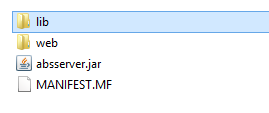
\includegraphics[width=0.6\textwidth]{img/abs-server.png}
    \caption{ABS Server yang sudah diarsipkan kedalam \texttt{.jar}}
    \label{fig:absServerJar}
\end{figure}

Sampai pada tahap ini penulis telah berhasil menghasilkan ABS MVC Framework yang dapat digunakan untuk membuat sebuah aplikasi web berbasis WEB beserta dengan ABS Server yang dapat digunakan untuk mencoba menjalankan aplikasi web yang telah dihasilkan.
\chapter{Penerapan ABS MVC Framework}

Bab ini membahas tentang penerapan ABS MVC Framework dalam pengembangan perangkat lunak berbasis web.

\section{Gambaran Umum Aplikasi Web}
Aplikasi web yang akan dibuat pada bab ini adalah aplikasi katalog produk yang fungsinya adalah untuk menyimpan dan menampilkan data tentang produk yang akan dijual di pasaran. Aplikasi web ini dibuat dengan tujuan untuk mendemonstrasikan tentang bagaimana membuat operasi \textit{create}, \textit{retrieve}, \textit{update} dan \textit{delete} (CRUD) dengan menggunakan ABS MVC Framework. Selain itu, penulis juga akan mendemonstrasikan bagaimana mengelola \textit{variability} degan pendekatan \textit{delta modelling} menggunakan ABS MVC Framework.\\

Berikut ini adalah fitur dari aplikasi web yang akan dibuat dengan menggunakan ABS MVC Framework:

\begin{enumerate}
    \item Menyimpan data produk (sku\footnote{\textit{stock keeping unit}, merupakan kode unik yang diberikan kepada setiap item sebagai bentuk identifikasi barang}, nama produk, deskripsi, harga).
    \item Menampilkan daftar produk.
    \item Mengubah data produk.
    \item Menghapus data produk.
\end{enumerate}

\section{Pembuatan Komponen Model}

Seperti yang sudah dibahas pada bab sebelumnya, komponen Model merupakan representasi dari data yang ada di dalam aplikasi. Dalam konteks aplikasi web yang akan dibuat, komponen Model ini akan merepresentasikan data produk yang yang akan disimpan oleh sistem dan ditampilkan kepada pengguna aplikasi. Pada tahap ini, penulis membuat sebuah modul ABS barus bernama \texttt{Product} dan menyimpan modul tersebut dengan nama \textit{Product.abs} di dalam direktori \texttt{src/abs/model} milik ABS MVC Framework.\\

Setelah selesai membuat modul baru, berikutnya adalah menuliskan kode ABS untuk mendefinisikan modul \texttt{Product} tersebut. Berikut ini adalah kode yang harus ditulis di dalam modul \texttt{Product}:

\begin{lstlisting}[
caption=Kode ABS untuk mendefinisikan komponen Model \texttt{Product},
label={lst:absProductModel},
escapeinside={@}{@}
]
module Model.Product;
export *;

interface Product
{
	String getSku(); @\label{lst:modelAccessor}@
	String getName();
	String getDescription();
	String getPrice();
	Unit setSku(String sku); @\label{lst:modelMutator}@
	Unit setName(String name);
	Unit setDescription(String description);
	Unit setPrice(String price);
}

class ProductImpl 
	(String sku, String name, String description, String price) implements Product
{
	String getSku() { return this.sku; }
	String getName() { return this.name; }
	String getDescription() { return this.description; }
	String getPrice() { return this.price; }
	Unit setSku(String sku) { this.sku = sku; }
	Unit setName(String name) { this.name = name; }
	Unit setDescription(String description) { this.description = description; }
	Unit setPrice(String price) { this.price = price; }
}
\end{lstlisting}

Seperti yang terlihat pada kode \ref{lst:absProductModel} di atas, konten dari \texttt{Product} hanya berisi atribut-atribut data seperti "sku", "name", "description", dan "price" beserta \textit{method} aksesor (\texttt{getSku()}) dan mutatornya (\texttt{setSku()}). Satu hal yang harus diperhatikan dalam mendefinisikan komponen Model ini adalah konvensi penamaan untuk \textit{method} aksesor dan mutatornya. Konvensi penamaan yang digunakan pada \textit{framework} ini adalah dengan memberikan prefix \texttt{set} untuk mutator dan \texttt{get} untuk aksesor yang kemudian diikuti dengan nama atribut dengan menggunakan format \textit{camel case} (lihat baris \ref{lst:modelAccessor} dan \ref{lst:modelMutator}). Konvensi ini ditujukan agar komponen Model yang dibuat dapat dikenali oleh Thymeleaf.\\

Setelah selesai membuat komponen Model, selanjutnya adalah membuat modul bantuan yang akan digunakan untuk mensimulasikan basis data pada aplikasi. Hal ini dilakukan karena ABS MVC Framework yang digunakan belum dapat mengakses basis data secara langsung seperti yang sudah disebutkan pada bagian batasan penelitian. Operasi-operasi yang dimiliki oleh modul ini antara lain adalah:

\begin{enumerate}
    \item \texttt{save}: operasi ini digunakan untuk menyimpan data produk yang diberikan.
    \item \texttt{delete}: operasi ini digunakan untuk menghapus data produk tertentu.
    \item \texttt{findAll}: operasi ini digunakan untuk mendapatkan seluruh data produk yang tersimpan.
    \item \texttt{findBySku}: operasi ini digunakan untuk mendapatkan data produk sesuai dengan kode SKU yang diberikan.
\end{enumerate}

Pada tahap ini penulis membuat sebuah modul baru yang bernama \texttt{ProductDB} yang kemudian disimpan ke dalam direktori \texttt{src/abs/model} dengan nama \texttt{ProductDB.abs}. Berikut ini adalah konten dari module \texttt{ProductDB.abs}:

\begin{lstlisting}[
caption=Kode ABS untuk modul \texttt{ProductDB},
label={lst:absProductDB},
escapeinside={@}{@}
]
module Model.ProductDB;
export *;
import Product, ProductImpl from Model.Product;

interface ProductDB
{
	Unit init();
	List<Product> findAll();
	Product findBySku(String sku);
	Unit save(Product obj);
	List<Product> delete(Product obj);
}

class ProductDBImpl implements ProductDB
{
	List<Product> db = Nil; @\label{lst:absProductList}@
	
	Unit init() @\label{lst:absProductDBInit}@
	{
		Product p1 = new local ProductImpl(
			"WH001", "LED TV 24' ", "FMSE LED TV 24 inch with 2 HDMI", "2.500.000");
			
		Product p2 = new local ProductImpl(
			"WH002", "LED TV 24' ", "FMSE LED TV 24 inch with 2 HDMI", "4.500.000");
			
		Product p3 = new local ProductImpl(
			"WH003", "Rice Cooker", "FMSE Electric Rice Cooker 5 litre", "1.500.000");
			
		db = appendright(db, p1);
		db = appendright(db, p2);
		db = appendright(db, p3);
	}
	
	List<Product> findAll()
	{
		return db;
	}
	
	Product findBySku(String sku)
	{
		Product result = null;
		Int index = 0;
		
		while(index < length(db))
		{
			Product current = nth(db, index);
			String currentSku = current.getSku();
			
			if(currentSku == sku)
			{
				result = current;
			}
			
			index = index + 1;	
		}
		
		return result;
	}
	
	Unit save(Product obj)
	{
		db = appendright(db, obj);
	}
	
	List<Product> delete(Product obj)
	{
		db = without(db, obj);
		
		return db;
	}
}
\end{lstlisting}

Seperti yang terlihat pada kode \ref{lst:absProductDB} baris \ref{lst:absProductList} diatas, penulis membuat sebuah \texttt{List<Product>} yang digunakan untuk menyimpan seluruh data produk. Setiap operasi-operasi yang ada di dalam modul \texttt{ProductDB} ini nantinya akan menggunakan \texttt{List<Product>} tersebut sebagai sumber datanya.\\

Untuk keperluan pengembangan aplikasi web yang dibuat, penulis membuat tiga buah data \textit{dummy} sebagai data awalan yang kemudian dimasukan kedalam \texttt{List<Product>} yang telah dibuat. Data awalan tersebut dibuat di dalam sebuah \textit{method} khusus bernama \textit{init} (lihat kode \ref{lst:absProductDB} baris \ref{lst:absProductDBInit}) yang akan dipanggil setiap kali melakukan inisialisasi modul ini. Dengan menggunakan pendekatan ini, penulis dapat mensimulasikan proses \textit{create}, \textit{retrieve}, \textit{update} dan \textit{delete} pada aplikasi web yang dibuat.

\section{Pembuatan Komponen View}

Setelah selesai membuat komponen Model, langkah berikutnya adalah membuat komponen View. Pada pengembangan aplikasi web ini, terdapat empat buah halaman HTML yang menjadi komponen View-nya. Keempat halaman tersebut harus disimpan kedalam folder \texttt{src/abs/view/product} agar dapat dikenali oleh ABS MVC Framework. Berikut ini adalah daftar berkas HTML yang harus dibuat berikut dengan kodenya:

\begin{enumerate}
    \item \texttt{index.html}: merupakan halaman web utama aplikasi yang berisi informasi tentang penggunaan sistem.
    \item \texttt{form.html}: merupakan halaman web yang digunakan untuk membuat produk baru.
    \item \texttt{update.html}: merupakan halaman web yang digunakan untuk mengubah data produk.
    \item \texttt{list.html}: merupakan halaman web yang berisi daftar produk dalam bentuk tabel.
\end{enumerate}

\subsection{Komponen View \texttt{index.html}}
Halaman HTML ini berfungsi sebagai halaman depan aplikasi yang berisikan informasi gambaran umum sistem dan cara penggunaannya. berikut ini adalah kode HTML yang harus dimasukan kedalam berkas \texttt{index.html}:

\begin{lstlisting}[
caption=Kode HTML untuk halaman \texttt{index.html},
label={lst:htmlIndex}
]
<!DOCTYPE html>
<html>
	<head>
		<title>Aplikasi Katalog Produk</title>
	</head>
<body>
	<div>
		<a href="/product/index.abs">Home</a> |
		<a href="/product/add.abs">Add Product</a> |
		<a href="/product/list.abs">Product List</a> |
	</div>
	<h4>Selamat Datang di Aplikasi Katalog Produk</h4>
	<p>Berikut ini adala fitur yang dapat digunakan:</p>
	<ul>
		<li>Untuk menambahkan data produk, silahkan klik menu "Add Product"</li>
		<li>Untuk Melihat daftar produk, silahkan klik menu "Product List"</li>
	</ul>
</body>
</html>
\end{lstlisting}

\subsection{Komponen View \texttt{form.html}}
Halaman HTML ini berisikan \texttt{HTML Form} yang digunakan untuk memasukan data produk baru kedalam sistem. berikut ini adalah kode HTML yang harus dimasukan kedalam berkas \texttt{form.html}:

\begin{lstlisting}[
caption=Kode HTML untuk halaman \texttt{form.html},
label={lst:htmlProductForm},
]
<!DOCTYPE html>
<html>
	<head>
		<title>Add Product</title>
	</head>
<body>
	<div>
		<a href="/product/index.abs">Home</a> |
		<a href="/product/add.abs">Add Product</a> |
		<a href="/product/list.abs">Product List</a> |
	</div>
	<h3>Product Details</h3>
	<form method="POST" action="/product/saveData.abs">
	<table>
		<tbody>
			<tr>
				<td>Product SKU</td>
				<td>:</td>
				<td><input type="text" name="product_sku"/></td>
			</tr>
			<tr>
				<td>Product Name</td>
				<td>:</td>
				<td><input type="text" name="product_name"/></td>
			</tr>
			<tr>
				<td>Description</td>
				<td>:</td>
				<td><input type="text" name="description" /></td>
			</tr>
			<tr>
				<td>Price</td>
				<td>:</td>
				<td><input type="text" name="price" /></td>
			</tr>
		</tbody>
	</table>
	<input type="submit" value="Submit" />
	</form>
</body>
</html>
\end{lstlisting}

\subsection{Komponen View \texttt{update.html}}

HTML ini berfungsi untuk menampilkan data produk sesuai dengan \textit{input} (nomor SKU) yang diberikan. Melalui halaman ini juga, pengguna aplikasi dapat mengubah data produk tersebut sesuai dan kembali menyimpannya kedalam sistem. berikut ini adalah kode HTML yang harus dimasukan kedalam berkas \texttt{update.html}:

\begin{lstlisting}[
caption=Kode HTML untuk halaman \texttt{update.html},
label={lst:htmlUpdateProduct}
]
<!DOCTYPE html>
<html>
	<head>
		<title>Edit Product</title>
	</head>
<body>
	<div>
		<a href="/product/index.abs">Home</a> |
		<a href="/product/add.abs">Add Product</a> |
		<a href="/product/list.abs">Product List</a> |
	</div>
	<h3>Product Details: <span th:text="${data.sku}"></span></h3>
	<form method="POST" action="/product/saveUpdate.abs">
	<input type="hidden" name="product_sku" th:value="${data.sku}"/>
	<table>
		<tbody>
			<tr>
				<td>Product Name</td>
				<td>:</td>
				<td><input type="text" name="product_name" th:value="${data.name}"/></td>
			</tr>
			<tr>
				<td>Description</td>
				<td>:</td>
				<td><input type="text" name="description" th:value="${data.description}"/></td>
			</tr>
			<tr>
				<td>Price</td>
				<td>:</td>
				<td><input type="text" name="price" th:value="${data.price}"/></td>
			</tr>
		</tbody>
	</table>
	<input type="submit" value="Submit" />
	</form>
</body>
</html>
\end{lstlisting}

Seperti yang terlihat pada kode \ref{lst:htmlUpdateProduct} di atas, penulis menambahkan sintaks Thymeleaf pada halaman ini agar halaman HTML ini dapat menampilkan data produk yang diberikan. Pada halaman ini, penulis menggunakan dua jenis sintaks Thymeleaf yaitu \texttt{th:text} dan \texttt{th:value}. sintaks \texttt{th:text} digunakan untuk menampilkan data dalam bentuk teks, sedangkan \texttt{th:value} adalah untuk menampilkan data kedalam bentuk atribut \texttt{value=""} di dalam tag \texttt{<input>}. Dengan menggunakan dua buah sintaks tersebut penulis sudah dapat menampilkan data produk pada halaman \texttt{update.html}.

\subsection{Komponen View \texttt{list.html}}

Halaman web ini dibuat dengan tujuan untuk menampilkan daftar seluruh produk yang disimpan di simpan oleh aplikasi dalam bentuk \texttt{HTML Table}. Berikut ini adalah kode HTML yang harus dimasukan kedalam berkas \texttt{list.html}

\begin{lstlisting}[
caption=Kode HTML untuk halaman \texttt{list.html},
label={lst:htmlListProduct},
escapeinside={+}{+}
]
<!DOCTYPE html>
<html>
	<head>
		<title>Product List</title>
	</head>
<body>
	<div>
		<a href="/product/index.abs">Home</a> |
		<a href="/product/add.abs">Add Product</a> |
		<a href="/product/list.abs">Product List</a> |
	</div>
	<h3>Product List</h3>
	<table>
		<thead>
			<tr>
				<th>No.</th>
				<th>SKU</th>
				<th>Product Name</th>
				<th>Price</th>
				<th>Action</th>
			</tr>
		</thead>
		<tbody>
			<tr th:each="product: ${dataList}">
				<td th:text="${#ids.seq('')}"></td> +\label{lst:thymeSequence}+
				<td th:text="${product.sku}"></td>
				<td th:text="${product.name}"></td>
				<td th:text="${product.price}"></td>
				<td>
					<a th:href="@{http://localhost:8080/product/update.abs(sku=${product.sku})}">update</a>&nbsp;&nbsp; +\label{lst:thymeUrl}+
					<a th:href="@{http://localhost:8080/product/delete.abs(sku=${product.sku})}">delete</a> +\label{lst:thymeUrl2}+
				</td>
			</tr>
		</tbody>
	</table>
</body>
</html>
\end{lstlisting}

Seperti yang terlihat pada kode \ref{lst:htmlListProduct} diatas, penulis juga menambahkan sintaks Thymeleaf untuk dapat menampilkan data produk kedalam halaman web. Berbeda dengan kode \ref{lst:htmlUpdateProduct} (halaman \texttt{update.html}) yang telah dibuat sebelumnya, pada halaman ini penulis menggunakan dua buah sintaks Thymeleaf yang lain yaitu \texttt{\$\{\#ids.seq()\}} (baris \ref{lst:thymeSequence}) dan \texttt{@\{url(param)\}} (baris \ref{lst:thymeUrl} dan \ref{lst:thymeUrl2}). Sintaks \texttt{\$\{\#ids.seq()\}} digunakan untuk menampilkan \textit{sequence id} seperti 1,2,3 dan seterusnya. Sedangkan sintaks \texttt{@\{url(param)\}} digunakan untuk menghasilkan dengan parameter seperti (\texttt{update.abs?sku=WH001}).

\section{Pembuatan Komponen Controller}
\chapter{Penerapan Delta Modelling Pada ABS MVC Framework}

Bab ini memaparkan tentang bagaimana menerapkan proses \textit{delta modelling} pada ABS MVC Framework. Dalam pemaparannya, penulis mengkaitkan proses penerapan \textit{delta modelling} tersebut dengan aplikasi web katalog produk yang telah dibuat sebelumnya. Adapun poin-poin yang akan dibahas pada bab ini antara lain adalah Perubahan \textit{requirement} pada aplikasi, Implementasi perubahan menggunakan \textit{delta code} dan Kompilasi dan \textit{deployment} varian produk.

\section{Perubahan \textit{requirement} pada aplikasi}
Pada dasarnya, fitur \textit{delta modelling} yang dimiliki oleh ABS dapat digunakan sebagai salah satu metode dalam menangani perubahan \textit{requirement} pada perangkat lunak. Untuk dapat memberikan gambaran terkait penerapan \textit{delta modelling} pada ABS MVC Framwork, penulis membuat sebuah perubahan \textit{requirement} pada aplikasi katalog produk yang telah dibuat sebelumnya. Adapun perubahan \textit{requirement} tersebut meliputi:

\begin{enumerate}
    \item Penambahan atribut kategori pada komponen model produk.
    \item Perubahan pada halaman tambah produk dengan menambahkan pilihan kategori produk yang terdiri dari "Electronic", "Cookware" dan "Furniture".
    \item Perubahan pada halaman daftar produk dengan menampilkan kategori produk pada tabel.
\end{enumerate}

\section{Implementasi perubahan menggunakan \textit{delta code}}
Setelah mendefinisikan perubahan \textit{requirement} pada aplikasi katalog produk, berikutnya adalah menerapkan perubahan tersebut dengan menggunakan pendekatan \textit{delta modelling} pada ABS MVC Framework. Dalam konteks ABS MVC Framework, penerapan \textit{delta modelling} tersebut dapat dilakukan pada komponen Model dan Controller yang dibuat dengan menggunakan ABS sedangkan pada komponen View harus dilakukan dengan cara membuat komponen baru sesuai dengan \textit{requirement} yang baru. Berikut ini adalah detail dari penerapan \textit{delta modelling} pada ABS MVC Framework.

\subsection{Pembuatan \textit{delta code} untuk komponen Model}

Seperti yang sudah disebutkan pada bagian perubahan \textit{requirement} pada aplikasi, perubahan aplikasi meliputi penembahan atribut kategori pada produk .Komponen model \texttt{Product} yang ada saat ini hanya memiliki atribut \texttt{sku}, \texttt{name}, \texttt{description} dan \texttt{price}. Agar komponen model yang ada sesuai dengan \textit{requirement} yang diinginkan, maka penulis perlu menambahkan satu buah atribut tambahan yang bernama \texttt{category} pada modul \texttt{Product} tersebut.\\

Untuk dapat melakukan perubahan yang diinginkan dengan menggunakan metode \textit{delta modelling}, penulis membuat sebuah modul ABS baru bernama \texttt{DProductModel} yang disimpan kedalam direktori \texttt{src/abs/delta} dengan nama \texttt{DProductModel.abs}. Berikut ini adalah kode ABS yang penulis buat untuk modul tersebut.

\begin{lstlisting}[
caption=Kode ABS Delta untuk komponen \texttt{ProductModel},
label={lst:deltaProductModel},
escapeinside={@}{@}
]
module Delta.ProductModel;

delta DProductModel; @\label{lst:absDefineDelta}@
uses Model.Product; @\label{lst:absDeltaUseModule}@

modifies interface Product @\label{lst:absDeltaModifyInterface}@
{
	adds String getCategory();
	adds Unit setCategory(String category);
}

modifies class ProductImpl @\label{lst:absDeltaModifyClass}@
{
	adds String category = ""; @\label{lst:absAddNewAttribute}@
	adds String getCategory() { return this.category; }
	adds Unit setCategory(String category) { this.category = category; }
}
\end{lstlisting}

Seperti yang terlihat pada kode \ref{lst:deltaProductModel} diatas, penulis membuat sebuah \textit{delta code} untuk modul \texttt{Product} (komponen Model) yang sudah dibuat pada bab penerapan ABS MVC Framework sebelumnya. Apa yang dilakukan oleh modul \texttt{DProductModel} tersebut adalah memodifikasi \texttt{interface Product} (baris \ref{lst:absDeltaModifyInterface}) dan \texttt{class ProductImpl} (baris \ref{lst:absDeltaModifyClass}) dengan menambahkan dua buah \textit{method} barus yaitu \texttt{getCategory} dan \texttt{setCategory}. Selain menambahkan kedua method tersebut \textit{method}, penulis juga menambahkan sebuah atribut baru yaitu \texttt{category} yang bertipe \texttt{String} seperti yang terlihat pada kode \ref{lst:deltaProductModel} baris \ref{lst:absAddNewAttribute} diatas.\\

Selain melakukan perubahan pada modul \texttt{Product}, penulis juga melakukan perubahan pada modul \texttt{ProductDB}. Perubahan yang dilakukan meliputi perubahan pada implementasi \textit{method} \texttt{init} yang bertugas dalam membuat data produk \textit{dummy} untuk aplikasi katalog produk yang dibuat. Hal ini perlu dilakukan untuk menyesuaikan implementasi komponen model \texttt{Product} yang berubah melalui kode delta yang dibuat sebelumnya. Dalam membuat kode delta untuk modul \texttt{ProductDB}, penulis membuat sebuah modul baru bernama \texttt{DProductDB} yang disimpan di dalam direktori \texttt{src/abs/delta} dengan nama berkan \texttt{DProductDB.abs}. Berikut ini adalah kode delta yang penulis buat pada modul \texttt{DProductDB} tersebut.

\begin{lstlisting}[
caption=Kode delta pada modul \texttt{DProductDB},
label={lst:deltaProductDB},
escapeinside={@}{@}
]
module Delta.ProductDB;

delta DProductDB;
uses Model.ProductDB;

modifies class ProductDBImpl
{
	modifies Unit init()
	{
		Product p1 = new local ProductImpl();
		p1.setSku("WH001");
		p1.setName("LED TV 24'");
		p1.setCategory("Electronic"); @\label{lst:deltaSetCategory}@
		p1.setDescription("FMSE LED TV 24 inch with 2 HDMI");
		p1.setPrice("2.500.000");

		Product p2 = new local ProductImpl();
		p2.setSku("WH003");
		p2.setName("Rice Cooker");
		p2.setCategory("Electronic"); @\label{lst:deltaSetCategory2}@
		p2.setDescription("FMSE Electric Rice Cooker 5 litre");
		p2.setPrice("1.500.000");
		
		Product p3 = new local ProductImpl();
		p3.setSku("WH004");
		p3.setName("Air Conditioner 1PK");
		p3.setCategory("Electronic"); @\label{lst:deltaSetCategory3}@
		p3.setDescription("FMSE Air Conditioner 1PK");
		p3.setPrice("4.500.000");
		
		db = appendright(db, p1);
		db = appendright(db, p2);
		db = appendright(db, p3);
	}
}
\end{lstlisting}

Kode \ref{lst:deltaProductDB} diatas tidak jauh berbeda dengan kode modul \texttt{ProductDB} yang telah paparkan pada bab penerapan ABS MVC Framework sebelumnya (kode \ref{lst:absProductDB}). Satu hal yang membedakan kode \ref{lst:deltaProductDB} dengan kode \ref{lst:absProductDB} sebelumnya terletak pada penambahan \textit{method} \texttt{setCategory} dalam melakukan pembuatan objek \texttt{Product} seperti yang terlihat pada baris \ref{lst:deltaSetCategory}, \ref{lst:deltaSetCategory2} dan \ref{lst:deltaSetCategory3}. Dalam kasus pembuatan kode delta untuk modul \texttt{ProductDB}, penulis harus melakukan implementasi ulang untuk \textit{method} \texttt{init} dikarenakan kode delta pada ABS tidak dapat digunakan untuk mengubah bagian kode di dalam \textit{method} secara spesifik.

\subsection{Pembuatan \textit{delta code} untuk komponen Controller}

Setelah membuat \textit{delta code} untuk modul \texttt{Product}, berikutnya penulis melakukan hal yang sama untuk modul \texttt{ProductController}. Hal ini dilakukan karena perubahan \textit{requirement} yang ada juga juga berdampak pada implementasi modul \texttt{ProductController} seperti misalnya menambahkan atribut kategori pada saat menyimpan dan memutakhirkan data produk yang diberikan oleh pengguna aplikasi. Oleh karena itu penulis juga membuat sebuah modul delta baru bernama \texttt{DProductController} yang disimpan di dalam direktori \texttt{src/abs/delta} dengan nama \texttt{DProductCoontroller.abs}. Berikut ini adalah kode delta yang penulis buat didalam modul tersebut.

\begin{lstlisting}[
caption=Struktur \textit{delta code} \texttt{DProductController},
label={lst:deltaProductController}
]
module Delta.ProductController;

delta DProductController;
uses Controller.Product;

modifies class ProductControllerImpl
{
	modifies Pair<String, List<Product>> productList(ABSHttpRequest request)
	{
		//detail implementasi kode delta
	}
	
	modifies Pair<String, List<Product>> updateProduct(ABSHttpRequest request)
	{
	    //detail implementasi kode delta	
	}
	
	modifies Pair<String, List<Product>> saveUpdateProduct(ABSHttpRequest request)
	{
		//detail implementasi kode delta
	}
	
	modifies Pair<String, List<Product>> addProduct(ABSHttpRequest request)
	{	
		//detail implementasi kode delta
	}
	
	modifies Pair<String, List<Product>> saveDataProduct(ABSHttpRequest request)
	{
		//detail implementasi kode delta
	}
	
	modifies Pair<String, List<Product>> deleteProduct(ABSHttpRequest request)
	{
		//detail implementasi kode delta
	}
}
\end{lstlisting}

Kode \ref{lst:deltaProductController} diatas merupakan \textit{skeleton} dari kode delta yang penulis buat untuk modul \texttt{ProductController}. Pada kode tersebut terlihat bahwa penulis melakukan modifikasi pada \textit{method} \texttt{productList}, \texttt{updateProduct}, \texttt{saveUpdateProduct}, \texttt{addProduct}, \texttt{saveDataProduct} dan \texttt{deleteProduct}. Berikut ini adalah detail modifikasi \textit{method} yang penulis buat pada modul \texttt{DProductController}.

\begin{lstlisting}[
caption=Kode delta untuk \textit{method} \texttt{addProduct},
label={lst:deltaAddProduct}
]
modifies Pair<String, List<Product>> addProduct(ABSHttpRequest request)
{	
	return Pair("product/withCategory/form", Nil);
}
\end{lstlisting}

Kode \ref{lst:deltaAddProduct} diatas merupakan kode delta yang dibuat untuk memodifikasi \textit{method} \texttt{addProduct} pada modul \texttt{ProductController}. Seperti yang terlihat pada kode tersebut, penulis hanya mengubah lokasi halaman HTML yang digunakan dari yang sebelumnya bertempat di \texttt{product/form} menjadi \texttt{product/withCategory/form} (yang sudah memiliki \textit{drop down} untuk kategori produk). Perubahan ini dilakukan karena \textit{method} \texttt{addProduct} hanya bertugas untuk menampilkan halaman untuk menambah produk tanpa ada proses lainnya.

\begin{lstlisting}[
caption=Kode delta untuk \textit{method} \texttt{updateProduct},
label={lst:deltaUpdateProduct}
]
modifies Pair<String, List<Product>> updateProduct(ABSHttpRequest request)
{
	Pair<String, List<Product>> originalResult = core.original(request);
	List<Product> productList = snd(originalResult);
	
	return Pair("product/withCategory/update", productList);
}
\end{lstlisting}

Kode \ref{lst:deltaUpdateProduct} diatas merupakan kode delta untuk \textit{method} updateProduct. Secara umum, apa yang penulis lakukan dengan menggunakan kode delta tersebut adalah mencoba untuk mengubah lokasi halaman HTML yang digunakan dari yang sebelumnya menggunakan berkas di \texttt{product/update} menjadi \texttt{product/withCategory/update} (yang sudah ditambahkan \textit{drop down} untuk kategori produk).Berbeda dengan kode delta yang penulis buat untuk \textit{method} \texttt{addProduct}, walaupun tujuan yang ingin dicapai sama yaitu mengganti halaman HTML yang digunakan namun pendekatan yang penulis lakukan berbeda. Hal ini terjadi dikarenakan pada \textit{method} \texttt{updateProduct} terdapat pemrosesan \textit{input} dan pencarian data produk di dalam \texttt{ProductDB} terlebih dahulu sebelum memberikan hasilnya ke \textit{web server}.\\

Pada kode \ref{lst:deltaUpdateProduct} tersebut, penulis melakukan pemanggilan \textit{method} \texttt{core.original()} yang merupakan salah satu \textit{method} khusus milik ABS untuk memanggil \textit{method} \texttt{updateProduct} yang belum diubah oleh kode delta. Dengan menggunakan cara ini, penulis tidak perlu melakukan implementasi ulang pada kode delta tersebut melainkan hanya mengambil nilai \texttt{List<Product>} yang dihasilkan dari \texttt{method} \texttt{updateProduct} yang asli untuk kemudian disematkan dengan halaman HTML yang baru.

\begin{lstlisting}[
caption=Kode delta untuk \textit{method} \texttt{productList},
label={lst:deltaProductList}
]
modifies Pair<String, List<Product>> productList(ABSHttpRequest request)
{
	Pair<String, List<Product>> originalResult = core.original(request);
	List<Product> productList = snd(originalResult);
	
	return Pair("product/withCategory/list", productList);
}
\end{lstlisting}

Kode \ref{lst:deltaProductList} diatas merupakan kode delta yang dibuat untuk memodifikasi implementasi \textit{method} \texttt{productList} pada modul \texttt{ProductController}. Secara umum kode delta yang penulis buat tidak berbeda dengan kode delta untuk \textit{method} \texttt{updateProduct} yaitu melakukan pemanggilan \texttt{core.original()} untuk mendapatkan hasil dari implementasi yang asli untuk kemudian diubah lokasi halaman HTML-nya dari yang sebelumnya \texttt{product/list} menjadi \texttt{product/withCategory/list} yang sudah ditambahkan kolom kategori produk pada tabelnya.

\begin{lstlisting}[
caption=Kode delta untuk \textit{method} \texttt{deleteProduct},
label={lst:deltaDeleteProduct}
]
modifies Pair<String, List<Product>> deleteProduct(ABSHttpRequest request)
{
	Pair<String, List<Product>> originalResult = core.original(request);
	List<Product> productList = snd(originalResult);
	
	return Pair("product/withCategory/list", productList);
}
\end{lstlisting}

Kode \ref{lst:deltaDeleteProduct} diatas merupakan kode delta untuk \textit{method} \texttt{deleteProduct} pada modul \texttt{ProductController}. Secara umum kode delta tersebut mirip dengan kode delta yang penulis buat untuk \textit{method} \texttt{updateProduct} dan \texttt{productList} yaitu memanggil method aslinya dengan menggunakan \texttt{core.original()} dan mengubah berkas HTML yang digunakan sebelum mengembalikannya ke \textit{web server}.

\begin{lstlisting}[
caption=Kode delta untuk \textit{method} \texttt{saveUpdateProduct},
label={lst:deltaSaveUpdateProduct},
escapeinside={@}{@}
]
modifies Pair<String, List<Product>> saveUpdateProduct(ABSHttpRequest request)
{
	ProductDB db = new local ProductDBImpl();
	db.init();
	
	String sku = request.getInput("product_sku");
	String name = request.getInput("product_name");
	String category = request.getInput("category"); @\label{lst:deltaGetInput}@
	String description = request.getInput("description");
	String price = request.getInput("price");
	
	Product p = db.findBySku(sku);
	p.setName(name);
	p.setCategory(category); @\label{lst:deltaAddSetCategory}@
	p.setDescription(description);
	p.setPrice(price);
	db.update(p);
	
	List<Product> products = db.findAll();
	return Pair("product/withCategory/list", products);
}
\end{lstlisting}

Kode \ref{lst:deltaSaveUpdateProduct} diatas merupakan kode delta yang ditujukan untuk memodifikasi \textit{method} \texttt{saveUpdateProduct} pada modul \texttt{ProductController}. Seperti yang terlihat pada kode delta tersebut, penulis melakukan implementasi ulang terhadap \textit{method} \texttt{saveUpdateProduct} tidak seperti kode delta untuk \texttt{updateProduct}, \texttt{deleteProduct} dan \texttt{productList} yang hanya melakukan pemanggilan \texttt{core.original}. Hal ini dilakukan karena penulis tidak hanya mengganti halaman HTML yang digunakan melainkan juga menambahkan beberapa baris kode seperti \texttt{request.getInput("category")} (baris \ref{lst:deltaGetInput}) dan \texttt{p.setCategory(category)} (baris \ref{lst:deltaAddSetCategory}).

\begin{lstlisting}[
caption=Kode delta untuk \textit{method} \texttt{saveDataProduct},
label={lst:deltaSaveDataProduct}
]
modifies Pair<String, List<Product>> saveDataProduct(ABSHttpRequest request)
{
	ProductDB db = new local ProductDBImpl();
	db.init();
	
	String sku = request.getInput("product_sku");
	String name = request.getInput("product_name");
	String category = request.getInput("category");
	String description = request.getInput("description");
	String price = request.getInput("price");
	
	Product p = new local ProductImpl();
	p.setSku(sku);
	p.setName(name);
	p.setCategory(category);
	p.setDescription(description);
	p.setPrice(price);
	
	db.save(p);
	
	List<Product> dataList = db.findAll();
	return Pair("product/withCategory/list", dataList);
}
\end{lstlisting}

Kode \ref{lst:deltaSaveDataProduct} diatas merupakan kode delta yang dibuat dengan tujuan untuk melakukan modifikasi pada \textit{method} \texttt{saveDataProduct}. Secara umum kode delta tersebut mirip dengan kode delta untuk \textit{method} \texttt{saveUpdateProduct} (kode \ref{lst:deltaSaveUpdateProduct}) yaitu melakukan implementasi ulang \textit{method} aslinya. Hal ini dilaukan karena selain mengubah halaman HTMLnya, penulis juga melakukan penambahan baris kode seperti yang penulis lakukan pada kode delta \ref{lst:deltaSaveUpdateProduct} yang sudah dipaparkan sebelumnya.

\section{Kompilasi dan \textit{deployment} varian produk}
\chapter{Evaluasi dan Analisa ABS MVC Framework}

Bab ini berisi tentang hasil analisis dan evaluasi dari MVC Framework yang telah dibuat. Dalam melakukan proses evaluasi, penulis membandingkan proses yang dilakukan dalam membuat perangkat lunak berbasis web antara menggunakan ABS MVC Framework dengan menggunakan framework lain. Adapun aplikasi web yang digunakan dalam proses evaluasi ini adalah aplikasi web yang telah penulis buat pada bagian penerapan ABS MVC Framwork (aplikasi katalog produk). Framework lain yang penulis gunakan dalam proses evaluasi ini adalah Play Framework (JAVA MVC Framework) versi 2.3 \footnote{https://playframework.com/download}. Berikut ini adalah poin-poin yang akan dievaluasi pada bab ini:

\begin{enumerate}
    \item Evaluasi proses penerapan Model-View-Controller.
    \item Evaluasi proses penanganan perubahan \textit{requirement}.
    \item Evaluasi penerapan SPL dengan menggunakan ABS MVC Framework.
\end{enumerate}

\section{Evaluasi Penerapan Model-View-Controller}

Dalam proses pengembangan apalikasi web dengan menggunakan MVC \textit{framework}, setiap kode yang dibuat akan dikelompokan kedalam komponen Model-View-Controller. Oleh karena itu, untuk mengevalusi framework ABS MVC yang dibuat penulis membandingan proses pembuatan komponen-komponen MVC tersebut antara Play Framework dengan ABS MVC Framework. Berikut adalah hasil evaluasi dan analisa ABS MVC Framework dari poin penerapan MVC-nya.

\subsection{Proses Pembuatan Komponen Model}

Komponen model merupakan komponen yang merepresentasikan entitas data pada aplikasi. Dalam banyak MVC Framework, komponen model dapat diintegrasikan dengan peragkat lunak basis data sehingga setiap komponen model yang dibuat akan merepresentasikan setiap tabel yang ada di dalam basis data. Dalam konteks ABS MVC Framework, proses integrasi komponen model dengan perangkat lunak basis data belum dapat dilakukan seperti yang sudah dibahas pada bagian batasan penelitian. Berikut ini adalah perbandingan antara komponen Model yang dibuat dengan menggunakan ABS MVC Framework dengan Play Framework.

\begin{lstlisting}[
caption=Komponen Model menggunakan ABS,
label={lst:modelUsingABS}
]
interface Product
{
    ...
}

class ProductImpl 
	(String sku, String name, String description, String price) implements Product
{
	String getSku() { return this.sku; }
	String getName() { return this.name; }
	String getDescription() { return this.description; }
	String getPrice() { return this.price; }
	Unit setSku(String sku) { this.sku = sku; }
	Unit setName(String name) { this.name = name; }
	Unit setDescription(String description) { this.description = description; }
	Unit setPrice(String price) { this.price = price; }
}
\end{lstlisting}

\begin{lstlisting}[
caption=Komponen Model menggunakan Play Framework,
label={lst:modelUsingPlay},
escapeinside={!}{!}
]
@Entity !\label{lst:modelAnotasi}!
public class Product extends Model
{
	@Id !\label{lst:modelAnotasi2}!
	public Long id;
	public String sku;
	public String name;
	public String description;
	public Long price;

	public Product(String sku, String name,
		String description, Long price)
	{
		this.sku = sku;
		this.name = name;
		this.description = description;
		this.price = price;
	}

	public static Finder<Long,Product> find = new Finder<Long,Product>( !\label{lst:modelPlayFinder}!
    Long.class, Product.class); 
}
\end{lstlisting}

Seperti yang terlihat pada Kode \ref{lst:modelUsingABS} dan \ref{lst:modelUsingPlay} diatas, kedua buah komponen Model tersebut tidak memiliki perbedaan yang signifikan. keduanya hanya berisikan atribut-atribut yang merepresentasikan data produk pada aplikasi web yang dibuat. Hanya saja, pada komponen model yang dibuat dengan menggunakan Play Framework memiliki tambahan anotasi (bari \ref{lst:modelAnotasi} dan \ref{lst:modelAnotasi2}) serta tambahan \textit{method} (baris \ref{lst:modelPlayFinder}) yang digunakan oleh Play Framework untuk mengintegrasikan komponen tersebut dengan perangkat lunak basis data.\\

Walaupun terdapat beberapa perbedaan antara komponen model yang dibuat dengan ABS Framework dengan Play Framework, akan tetapi kedua komponen tersebut masih memiliki karakteristik yang sama yaitu hanya terdiri dari atribut data dan tidak mengandung proses bisnis aplikasi. Hal ini sejalan dengan definisi komponen Model yang dipaparkan oleh \cite{krasner1988desc} dan \cite{leff2001web} pada publikasi penelitiannya. Dengan demikian, penulis berkesimpulan bahwa metode yang digunakan pada ABS MVC Framework sudah sesuai dengan karakteristik komponen model pada \textit{framework} yang umum digunakan dan juga sudah sesuai dengan landasan teori yang ada.

\subsection{Proses Pembuatan Komponen View}

Dalam banyak \textit{framework} MVC, pembuatan komponen View umumnya menggunakan sintaks HTML dengan tambahan sintaks \textit{template engine} untuk dapat mengintegrasikan antara komponen View tersebut dengan komponen Model yang dibuat. Dalam konteks ABS MVC Framework, komponen View yang dibuat sudah menggunakan sintaks HTML dan \textit{template engine} Thymeleaf sedangkan Play Framewerk juga sudah menggunakan HTML dan \textit{template engine} Twirl. Berikut ini adalah perbandingan komponen View yang dibuat dengan menggunakan ABS MVC Framework dan Play Framework.

\begin{lstlisting}[
caption=Halaman \texttt{list.html} yang dibuat menggunakan Thymeleaf,
label={lst:viewThymeleaf},
escapeinside={!}{!}
]
...
<tbody>
	<tr th:each="product: ${dataList}"> !\label{lst:thymeDataList}!
		<td th:text="${#ids.seq('')}"></td>
		<td th:text="${product.sku}"></td>
		<td th:text="${product.name}"></td>
		<td th:text="${product.price}"></td>
		<td>
			<a th:href="@{http://localhost:8080/product/update.abs(sku=${product.sku})}">update</a>&nbsp;&nbsp;
			<a th:href="@{http://localhost:8080/product/delete.abs(sku=${product.sku})}">delete</a>
		</td>
	</tr>
</tbody>
...
\end{lstlisting}

\begin{lstlisting}[
caption=Halaman \texttt{list.html} yang dibuat menggunakan Twirl,
label={lst:viewTwirl},
escapeinside={!}{!}
]
@(products: List[Product]) !\label{lst:twirlDefineVariable}!
...
<tbody>
	@for((product, index) <- products.zipWithIndex){
		<tr>
			<td>@{index+1}</td>
			<td>@product.sku</td>
			<td>@product.name</td>
			<td>@product.price</td>
			<td>
				<a href="/product/update/@product.sku">update</a>&nbsp;&nbsp;
				<a href="/product/delete/@product.sku">delete</a>
			</td>
		</tr>
	}
</tbody>
...
\end{lstlisting}

Seperti yang terlihat pada Kode \ref{lst:viewThymeleaf} dan \ref{lst:viewTwirl}, kedua komponen View tersebut tidak jauh berbeda dikarenakan keduanya dibuat dengan menggunakan sintaks HTML. Hal yang membedakan dari kedua komponen tersebut terletak pada sintaks \textit{template engine} yang digunakan seperti misalnya pada ABS MVC Framework menggunakan \texttt{\$\{data.sku\}} untuk mendapatkan nomor sku dari objek model yang diberikan, sedangkan Play Framework menggunakan sintaks \texttt{@product.sku}. Perbedaan sintaks ini adalah wajar dikarenakan \textit{template engine} yang digunakan oleh kedua \textit{framework} tersebut adalah berbeda.\\

Walaupun kedua komponen di atas hampir sama, namum komponen View yang dibuat oleh komponen ABS MVC Framework banyak memiliki keterbatasan jika dibandingkan dengan komponen View yang dibuat dengan menggunakan Play Framework. berikut adalah beberapa keterbatasan yang dimiliki oleh ABS MVC Framework:

\begin{itemize}
    \item Memerlukan konvensi khusus untuk dapat memanggil komponen model yang diberikan seperti misalnya penggunaan variable \texttt{dataList} (Kode \ref{lst:viewThymeleaf} barsi \ref{lst:thymeDataList}) untuk objek model berbentuk list dan \texttt{data} (Kode \ref{lst:htmlUpdateProduct}) untuk objek model yang berdiri sendiri. Hal ini berbeda dengan komponen View pada Play Framework yang dapat didefinisikan sendiri oleh pengembang (Kode \ref{lst:viewTwirl} baris \ref{lst:twirlDefineVariable}).
    \item Komponen View pada ABS MVC Framework belum dapat menangani banyak komponen Model yang artinya ketika pengembang membuatuhkan Model Product dan Customer untuk ditampilkan di halaman web,  hal ini belum dapat dilakukan. Berbeda dengan komponen View pada Play Framework yang dapat menerima banyak model dengan menggunakan \texttt{@\(product: Product, customer: Customer\)}.
\end{itemize}

Berdasarkan hasil evaluasi diatas, penulis menyimpulkan bahwa untuk komponen View yang dibuat menggunakan ABS MVC Framework, sudah memiliki karakteristik yang sama dengan komponen yang dibuat menggunakan Play Framework. Akan tetapi, masih terdapat beberapa keterbatasan yang dimiliki sehingga tingkat fleksibilitasnya masih rendah dibandingkan dengan komponen View yang dibuat dengan menggunakan Play Framework.

\subsection{Proses Pembuatan Komponen Controller}

Secara umum fungsi dari komponen Controller adalah mengintegrasikan komponen Model dan View agar dapat dihasilkan sebuah halaman web yang dapat ditampilkan ke pengguna aplikasi. Dalam implementasinya, komponen Controller berisi bisnis proses aplikasi yang didalamnya melakukan pemrosesan \textit{input} yang diberikan oleh pengguna aplikasi. Dalam konteks ABS MVC Framework, kedua hal tersebut sudah dapat dilakukan walaupun dengan mekanisme yang sedikit berbeda dengan komponen Controller yang dibuat dengan menggunakan Play Framework. Berikut ini adalah cuplikan \textit{method} \texttt{saveUpdateProduct} yang ada di dalam Controller ABS MVC Framework dan Play Framework:

\begin{lstlisting}[
caption=Method \texttt{saveUpdateProduct} menggunakan ABS MVC Framework,
label={lst:saveUpdateABS}
]
...
Pair<String, List<Product>> saveUpdateProduct(ABSHttpRequest request)
{
	ProductDB db = new local ProductDBImpl();
	db.init();
	
	String sku = request.getInput("product_sku");
	String name = request.getInput("product_name");
	String description = request.getInput("description");
	String price = request.getInput("price");
	
	Product p = db.findBySku(sku);
	p.setName(name);
	p.setDescription(description);
	p.setPrice(price);
	db.update(p);
	
	List<Product> products = db.findAll();
	return Pair("product/list", products);
}
...
\end{lstlisting}

\begin{lstlisting}[
caption=Method \texttt{saveUpdateProduct} menggunakan Play Framework,
label={lst:saveUpdatePlay}
]
public static Result saveUpdateProduct()
{
    DynamicForm requestData = Form.form().bindFromRequest();
    String sku = requestData.get("product_sku");
    String name = requestData.get("product_name");
    String description = requestData.get("description");
    Long price = Long.parseLong(requestData.get("price"));

    List<Product> products = Product.find.where().eq("sku", sku).findList();
    Product product = products.get(0);
    product.name = name;
    product.description = description;
    product.price = price;
    product.update();

    return ok(list.render(Product.find.all()));
}
\end{lstlisting}

Seperti yang terlihat pada Kode \ref{lst:saveUpdateABS} dan \ref{lst:saveUpdatePlay} diatas, secara umum apa yang dilakukan oleh kedua buah \textit{method} tersebut adalah sama yaitu (1) menerima input dari pengguna aplikasi, (2) melakukan pencarian kedalam basis data untuk mendapatkan produk dengan nomor sku yang sesuai, (3) Mengubah data produk tersebut dengan data yang diberikan oleh pengguna aplikasi dan (4) menampilkan seluruh data produk kedalam halaman \texttt{list.html}. Satu hal yang membedakan kedua komponen Controller diatas adalah pada ABS MVC Framework basis data yang digunakan masih merupakan basis data \textit{dummy} sedangkan pada Play Framework, penulis sudah menggunakan MySQL sebagai basis datanya. Hal ini terjadi karena saat ini, ABS masih belum dapat melakukan akses kedalam basis data sungguhan seperti yang sudah dipaparkan pada bagian batasan penelitian.\\

Selain batasan terkait akses basis data tersebut, terdapat pula keterbatasan lainya yang dimiliki oleh ABS MVC Framework dalam membuat komponen Controller yaitu adalah belum adanya mekanisme yang dapat digunakan oleh ABS MVC Framework untuk memberikan banyak model kedalam komponen View. Hal ini menyebabkan adanya keterbatasan pada komponen View seperti yang dibahas pada bagian evaluasi pembuatan komponen View. Adanya keterbatasan pada komponen Controller dalam memberikan banyak model adalah karena penulis belum menemukan pengganti tipe data \texttt{Generic} yang dimiliki oleh JAVA untuk ABS.\\

Walaupun terdapat beberapa keterbatasan fitur pada komponen Controller ABS MVC Framework, akan tetapi secara karakteristik antara komponen Controller ABS MVC Framework dengan Play Framework tidak jauh berbeda. Sehingga dapat disimpulkan bahwa komponen Controller yang dibentuk dengan menggunakan ABS MVC Framework masih sesuai dengan karakteristik yang dipaparkan oleh \cite{krasner1988desc} dan \cite{leff2001web} serta \textit{framework} MVC lain yang biasa digunakan.

\section{Evaluasi Proses Penanganan Perubahan Requirement}

Perubahan \textit{requirement} terhadap sistem, merupakan satu hal yang tidak dapat dihindari. Dalam konteks ABS MVC Framework, perubahan \textit{requirement} terssebut dapat ditangani dengan membuat kode delta seperti yang penulis bahas pada bab sebelumnya. Dengan menggunakan pendekatan ini, setiap perubahan \textit{requirement} akan tercatat dalam bentuk kode delta yang dibuat sehingga para pengembang memiliki dokumentasi yang jelas terhadap setiap perubahan yang terjadi di dalam sistem. Selain itu, dengan menggunakan pendekatan \textit{delta modelling}, para pengembang aplikasi web dapat dengan leluasa memilih perubahan mana saja yang ingin diimplementasikan tanpa harus kehilangan aplikasi yang aslinya.\\

Lain halnya dengan menggunakan Play Framework, pada saat terjadi perubahan \textit{requirement} pada sistem, mau tidak mau para pengembang aplikasi web tersebut harus melakukan perubahan secara langsung terhadap setiap komponen Model, View dan Controller-nya. Hal ini tentunya akan menyebabkan hilangnya kode aplikasi yang sudah dibuat sebelumnya. Dengan menggunakan pendekatan ini, para pengembang aplikasi web tersebut tidak dapat melacak jejak perubahan yang terjadi pada perangkat lunak yang dibuat dikarenakan setiap perubahan yang terjadi pada sistem langsung berdampak pada kode asli pada sistem tersebut.\\

Berdasarkan pemaparan diatas, dapat diketahui bahwa proses penangan perubahan \textit{requirement} dengan menggunakan pendekatan \textit{delta modelling} memberikan dampak yang lebih baik dibandingkan dengan melakukan perubahan secara langsung terhadap kode aplikasi yang dibuat. Dengan demikian, penulis berpendapat bahwa dalam penangan perubahan \textit{requirement} ini ABS MVC Framework memiliki nilai lebih dibandingkan dengan Play Framework.

\section{Evaluasi penerapan SPL dengan menggunakan ABS MVC Framework}

\textit{Software Product Line Engineering} (SPLE) merupakan sebuah paradigma yang digunakan dalam proses pengembangan perangkat lunak dengan menggunakan prinsip \textit{platform} dan \textit{mass customisation} \citep[p.~14]{pohl2005software}. Dengan menggunakan paradigma ini, para pengembang perangkat lunak dapat menciptakan banyak variasi produk dari produk inti (\textit{core product}) yang dibuat dengan cara melakukan proses perubahan (\textit{customization}) pada produk tersebut. Dalam konteks ABS MVC Framework, proses pembuatan SPLE dapat dilakukan dengan menggunakan pendekatan \textit{delta modelling}. Dengan menggunakan pendekatan ini, para pengembang perangkat lunak dapat menerapkan prinsip \textit{platform} dengan cara membuat \textit{core product} menggunakan kode ABS dan prinsip \textit{mass customization} dengan cara membuat banyak kode delta yang nantinya akan diterapkan di dalam \textit{core product} tersebut untuk dapat menghasilkan banyak variasi produk / \textit{productline}.\\

Sebagai contoh, pada pembahasan sebelumnya penulis telah membuat sebuah perubahan \textit{requirement} pada aplikasi katalog produk yang penulis buat. Perubahan \textit{requirement} tersebut dapat dianggap sebagai sebuah variasi produk dari produk intinya yaitu sebuah aplikasi katalog produk dengan tanpa kategori produk di dalamnya. Dalam kasus ini, penulis memiliki sebuah \textit{productline} yaitu aplikasi web katalog produk yang menyertakan kategori produk di dalamnya. Apabila penulis ingin membuat \textit{productline} yang lain seperti misalnya menambahkan atribut "diskon" pada data produk, penulis cukup membuat kode delta lain dan menambahkannya kedalam konfigurasi produk untuk dapat menghasilkan variasi produk yang baru.\\

Berdasarkan pemaparan tersebut, dapat diketahui bahwa ABS MVC Framework dapat memfasilitasi para pengembang perangkat lunak dalam menghasilkan SPL untuk aplikasi web yang dibuat.
\chapter{Kesimpulan}

Berdasarkan hasil evaluasi yang penulis lakukan terhadap ABS MVC Framework, penulis membuat beberapa kesimpulan dari hasil penelitian ini yang diantaranya adalah:

\begin{enumerate}
    \item Pola pengembangan Model-View-Controller dapat diterapkan pada bahasa pemodelan ABS dengan menjadikan ABS sebagai komponen Model dan Controller-nya sedangkan HTML sebagai komponen View-nya. Dalam implementasinya, dibutuhkan adanya bantuan dari \textit{template engine} untuk mengintegrasikan komponen Model dengan komponen View yang dibuat.
    \item Fitur \textit{delta modelling} dapat diterapkan pada ABS MVC Framework dan digunakan untuk memodifikasi atau menambahkan komponen Model dan Controller pada \textit{framework} tersebut. Fitur \textit{delta modelling} tidak dapat diguanakan pada komponen View dikarenakan pada ABS MVC Framework komponen View tidak dibuat dengan menggunakan ABS melainkan HTML.
    \item Proses pengembangan SPL berbasis web dapat diterapkan dengan menggunakan ABS MVC Framework dengan cara menerapkan konsep \textit{delta modelling} pada aplikasi yang dibuat. Dalam konteks ABS MVC Framework, para pengembang perangkat lunak dapat membuat sebuah aplikasi web sebagai \textit{core product} dengan menggunakan ABS dan kemudian mebuat kode-kode delta serta konfigurasi produk yang nantinya akan diterapkan pada \textit{core product} yang dibuat untuk menghasilkan variasi produk yang diinginkan.
\end{enumerate}


\bibliography{conf/bib}
\bibliographystyle{conf/apalikerd}

\end{document}